\documentclass[11pt,a4paper]{article}
\usepackage[margin=2.3cm]{geometry}
\usepackage{amsmath,amssymb,graphicx,booktabs,array,microtype,xcolor,caption,float}
\usepackage[hidelinks]{hyperref}
\usepackage[authoryear,round]{natbib}
\captionsetup{font=small,labelfont=bf}
\newcommand{\Msun}{M_\odot}
\newcommand{\ftau}{M,R,f,\tau}

\title{Exploring the Limits of Machine-Learning Classification of Neutron-Star Matter Models:\\[2pt]
\large Populations of Equations of State, Illustrative Observational Errors and Calibrated Uncertainty}
\author{Wasif Husain\\ \small School of Science, Technology and Engineering, University of Sunshine Coast, Adelaide 5000}
\date{Revised manuscript (supersedes arXiv:2512.23758v3)}

\begin{document}
\maketitle

\begin{abstract}
Machine-learning classification of neutron-star composition is usually demonstrated on synthetic data in which every composition is a single equation of state (EoS) and test points are drawn along the same sequences. We show that the 97\% accuracy of such a released benchmark (770 models) is largely interpolation between neighbouring models, and replace it by a controlled identifiability study: 360 EoS, 90 in each of four phenomenological scenarios (nucleonic, hyperonic-like, strange, and neutron-decay dark-matter-admixed with the dark-fermion mass inside its stability window), each solved with a general-relativistic TOV, tidal and $f$-mode code written for this work. The code agrees to 0.007\% with six $f$-mode frequencies of an unpublished same-author pilot that shares the EoS inputs (a code-to-code consistency check, not an absolute accuracy), reproduces analytic benchmarks, and gives damping times 2.9--7.0\% above a published relation for nuclear EoS, a difference that is not understood.
With whole-EoS hold-out, six classifiers, their tuned variants and a kernel-Bayes reference reach only 65\% accuracy without measurement error (95\% bootstrap interval 61--67\%, conditional on the catalogue and classifiers). Strange matter is separable and hyperonic-like matter partly, but no discrimination between nucleonic and dark-matter-admixed matter is demonstrated (pairwise accuracy 51\%, interval 45--56\%). With the nuclear EoS known exactly the dark component shifts $f$ by a median of 0.57\% and an $f$-mode precision of about 0.51\% would be needed for 75\% detection; this shift depends on the baryon-number prescription of the one-fluid model (a change of $m_0$ to 938.9\,MeV alters it by a median of 5\% and at most 6\% inside the stability window, up to 65\% above it). When the nuclear parameters are confined to windows about a fiducial EoS, the nucleonic-versus-dark-matter accuracy stays near chance while the spread of $f$ among nuclear EoS exceeds about 1\% and reaches 81\% when it is 0.2\%, below the shift.
With illustrative errors taken from different published measurements (not a realistic joint observation) the accuracy is 33--37\% (chance 25\%) and conformal prediction sets contain 3.22 of four classes; their coverage (0.91--0.92 at the 0.90 target) is empirical, not guaranteed. An alternative population with different parametrisations again shows no demonstrated nucleonic--dark-matter discrimination but not the 65\% plateau. All results are conditional on the phenomenological families, priors and error models defined here; no inference about real stars is claimed.
\end{abstract}

\section{Introduction}
Neutron stars probe matter at densities well above nuclear saturation \citep{LP04,OF16}. Their composition is uncertain: purely nucleonic matter, matter containing hyperons, deconfined quark matter and, in speculative scenarios, an admixture of dark matter---for example from the decay of neutrons into a dark fermion \citep{FG18,Husain22}---have all been proposed. Observations constrain the equation of state (EoS) rather than the composition directly: pulsar masses, NICER measurements of masses and radii \citep{Riley19,Miller19} and the tidal deformability measured in GW170817 \citep{Abbott18}. Oscillation frequencies offer additional information (gravitational-wave asteroseismology; \citealt{AK98,Benhar04}), and the $f$-mode of stars containing neutron-decay dark matter has been studied by the author \citep{Husain25}. Dark matter in neutron stars has a large literature \citep[e.g.][]{Leung11,Ellis18}, and neutron-star masses strongly constrain neutron decay into dark fermions unless these interact repulsively \citep{Baym18,McKeen18,Motta18}, the case modelled here. Machine learning has been applied to map neutron-star observables to the EoS \citep{Fujimoto18,Ferreira21}.

A natural question, and the one addressed here, is how far a supervised classifier can distinguish \emph{composition} from observables, and where the answer is limited by physics rather than by the algorithm. A previous version of this work (arXiv:2512.23758v3) trained a small multilayer perceptron (MLP) on seven observables of 770 synthetic stellar models, each class being one EoS, and reported a test accuracy of 97.4\% on 116 held-out models. That number does not support the conclusions drawn from it (Sec.~\ref{sec:legacy}), and a single sequence per class cannot say how well compositions can be told apart when the EoS itself is uncertain. This revision replaces the benchmark by a controlled identifiability study and does the following.
\begin{enumerate}
\item \textbf{Re-examines the single-sequence benchmark} (Sec.~\ref{sec:legacy}, Appendix~\ref{sec:legacynoise}): class sizes, mass coverage, a class-dependent redshift inconsistency, and the dependence of the accuracy on how test points are chosen.
\item \textbf{Builds populations of EoS} for four composition scenarios and solves every EoS with a general-relativistic TOV, tidal and $f$-mode code written for this work (Sec.~\ref{sec:pop}). The code is checked against a same-author cross-code pilot, analytic benchmarks and a published damping-time relation, and the limits of these checks are stated.
\item \textbf{Evaluates with whole-EoS hold-out}, six learners (plus tuned variants and physically motivated features) and a kernel-Bayes reference classifier (Secs.~\ref{sec:methods}, \ref{sec:results}), under error scenarios taken from published measurements and forecasts---combined illustratively, not as a realistic joint observation---and on a precision scale that shows what accuracy of measurement would be required.
\item \textbf{Quantifies what limits the dark-matter signal}: its size at fixed nuclear EoS, its dependence on stellar mass and on the modelling prescription, and how the nucleonic-versus-dark-matter accuracy changes as the nuclear EoS is assumed to be known more precisely (Secs.~\ref{sec:paired}, \ref{sec:narrow}).
\item \textbf{Quantifies uncertainty and robustness}: calibration, conformal prediction sets calibrated at the level of whole EoS, EoS-level bootstrap intervals, and an alternative population with different parametrisations and priors (Secs.~\ref{sec:unc}--\ref{sec:popB}).
\end{enumerate}
\emph{Scope.} The EoS are phenomenological parametrisations with uniform priors, not microphysical calculations, and no real observations are used. All results are therefore conditional statements about the populations, priors and error models defined here, and about their identifiability, not inferences about real stars. Appendix~\ref{sec:changes} lists each claim of the earlier version that has been withdrawn or changed.

\section{Why a single sequence per class cannot answer the question}\label{sec:legacy}
The earlier version of this work released 770 synthetic stellar models (\texttt{DataML.xlsx}) in which each of four classes is one EoS. An audit of that data set (Appendix~\ref{sec:data}) shows that the classes contain 222, 220, 122 and 206 models; that the models lie on a regular radius grid, so that for 96.5\% of them the nearest neighbour in $(\ln M,\ln R,\ln f,\ln\tau)$ belongs to the same class; that 70\% of the models have $M<1\,\Msun$ and the dark-matter sequence ends at $0.68\,\Msun$; and that the tabulated surface redshift is inconsistent with $(M,R)$ for two classes in a way that alone separates the classes with 91\% cross-validated accuracy, so it is not used here. Repeating the random-split protocol (Appendix~\ref{sec:repro}) reproduces the published 97.4\% ($97.7\pm1.6\%$ over 100 seeds) but a random forest reaches 99.2\%, and removing the redshift changes the MLP result only to 97.5\%: the number is reproducible, but it is not specific to the method.

The decisive test holds out contiguous blocks of models (noise-free, 70/30 split, 15 repetitions; Fig.~\ref{fig:block}). With all six tabulated observables $(M,R,f,Q,\tau,h_c)$ the MLP accuracy falls from 97\% (single-model hold-out, equivalent to a random split) to 94\% for six-model blocks and 69\% for 24; the random forest falls from 99\% to 82\% and 42\%. With the four plausibly measurable observables $\ftau$ the MLP values are 78\%, 69\% and 45\%. A large part of the apparent skill is therefore interpolation between near-duplicate neighbours of the same sequence. $Q$ and $h_c$ are model-derived amplitudes rather than measurable quantities and are not used further.
\begin{figure}[t]\centering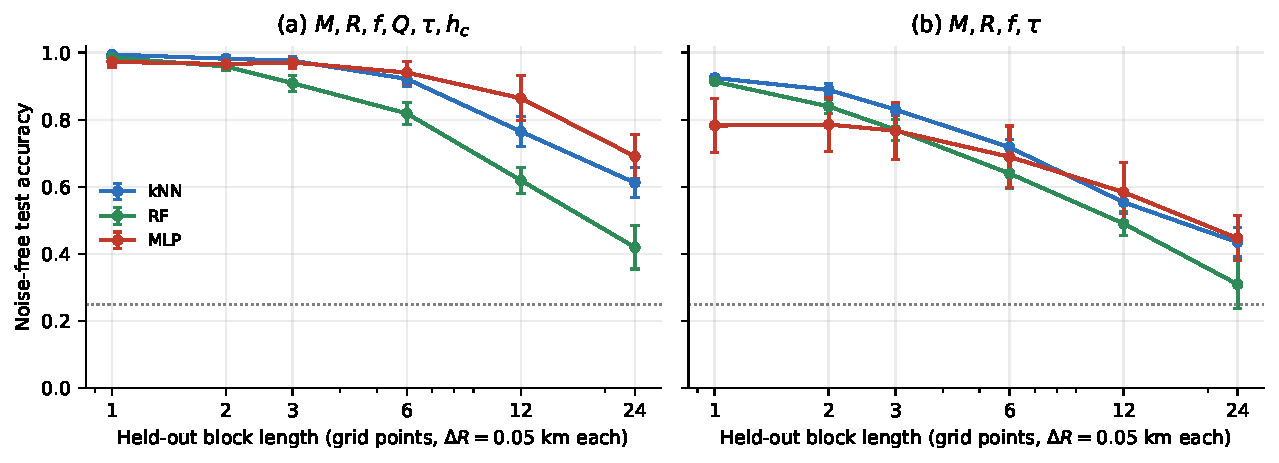
\includegraphics[width=.95\textwidth]{figs/fig3_blocksize.pdf}
\caption{Single-sequence benchmark: noise-free test accuracy versus the length of the held-out contiguous mass block (mean and 95\% $t$-interval over 15 repetitions). Dotted: chance. A block length of one is equivalent to the random split of the earlier version.}\label{fig:block}\end{figure}
Even with the leakage removed, a single sequence per class cannot say whether composition is identifiable when the EoS itself is uncertain: ``classifying the family'' and ``recognising one EoS'' are the same task. The remainder of the paper therefore studies \emph{populations} of EoS and holds out whole EoS.

\section{A population of equations of state}\label{sec:pop}
\subsection{Composition scenarios as EoS populations}
Each scenario is a family of EoS defined by a small number of parameters with a uniform prior (Table~\ref{tab:priors}); one draw from the prior is one EoS. The families are phenomenological parametrisations \emph{inspired by} the four scenarios of the earlier version, not microphysical calculations.
\begin{table}[t]\centering\small
\caption{Parametrisations and priors. PP: piecewise polytrope \citep{Read09} with core break densities $\rho_1=10^{14.7}$ and $\rho_2=10^{15}$\,g\,cm$^{-3}$ on a four-piece crust; CSS: constant speed of sound, $\varepsilon=\varepsilon_0+p/c_s^2$.}\label{tab:priors}
\begin{tabular}{>{\raggedright\arraybackslash}p{.17\textwidth}p{.75\textwidth}}\toprule
Scenario & Parameters (uniform priors)\\\midrule
Nucleonic & PP: $\log_{10}P_1\in[34.15,34.60]$ (dyn\,cm$^{-2}$ at $\rho_1$), $\Gamma_1\in[2.4,3.8]$, $\Gamma_2\in[2.4,3.9]$, $\Gamma_3\in[2.2,3.9]$\\
Hyperonic-like & PP with $\log_{10}P_1\in[34.20,34.60]$, $\Gamma_1\in[2.6,3.8]$ and a soft segment $\Gamma_2\in[1.8,2.6]$ above $\rho_1\approx2n_0$ (hyperon onset), then a causal CSS segment with $c_s^2\in[0.5,1]$ above $\rho_t=10^{u}$, $u\in[14.95,15.25]$\\
Strange (self-bound) & CSS with $\varepsilon_0=4B$, $B^{1/4}\in[130,160]$\,MeV, $c_s^2\in[1/3,1]$ ($c_s^2=1/3$ is the MIT bag model)\\
Dark-matter admixed & nucleonic PP prior plus a self-interacting dark Fermi gas in chemical equilibrium with the baryons (neutron-decay scenario): $m_\chi\in[937.9,938.783]$\,MeV (stability window), repulsive self-interaction $G\in[50,500]$\,fm$^2$; effective one-fluid barotrope\\\bottomrule\end{tabular}\end{table}
The dark-fermion mass window follows the neutron-decay dark-matter scenario \citep{FG18}: $m_\chi>937.9$\,MeV is required for the stability of $^{9}$Be and $m_\chi<m_p+m_e=938.783$\,MeV for the stability of $\chi$. Both bounds are imposed in the primary population, so every dark-matter EoS has $m_\chi$ inside the window. An earlier version of this analysis drew $m_\chi$ up to 939.2\,MeV, which exceeds the second bound for 27 of its 90 dark-matter EoS; that population is kept as a sensitivity run (Sec.~\ref{sec:robust}).
Draws are accepted only if they satisfy broad observational and consistency screens: $M_{\max}\ge1.97\,\Msun$, a causal speed of sound ($c_s^2\le1$) up to the centre of the maximum-mass star, $70\le\Lambda_{1.4}\le800$ and $10\le R_{1.4}\le14$\,km. The acceptance rates are 21\%, 57\%, 21\% and 26\% for the nucleonic, strange, dark-matter and hyperonic-like priors, so the screens remove most of the prior volume (mainly through $M_{\max}$ and causality, and for strange matter through $\Lambda_{1.4}$ and $R_{1.4}$). Observables are tabulated for stars of $1.2$--$1.9\,\Msun$ and evaluated on a mass grid over $1.2$--$1.85\,\Msun$, where all accepted EoS have stable stars.

The dark-matter-admixed scenario follows the effective-barotrope construction of the earlier work: baryons (nucleonic PP, $\mu_N=(\varepsilon+p)/n_B$) and a dark Fermi gas with $\mu_\chi=\sqrt{m_\chi^2+k_F^2}+\hbar cGn_\chi$ share one chemical potential, and the total pressure and energy density are summed at that potential. Because the dark component appears only above $\mu_N=m_\chi$, which in this construction happens at $\rho=1.1$--$1.7\times10^{11}$\,g\,cm$^{-3}$ (the outer crust, below neutron drip), the outermost layers are purely baryonic and the dark component is present throughout the rest of the star. Its share of the central energy density is small: a median of 0.94\% (maximum 4.6\%) at $1.4\,\Msun$ and 1.24\% (maximum 6.2\%) at $1.8\,\Msun$ over the 90 EoS. The onset density is a feature of the effective one-fluid construction (it depends on the baryon-number prescription discussed in Sec.~\ref{sec:paired}); it is not a prediction of a microscopic neutron-decay calculation. By construction this scenario shares the nuclear prior with the nucleonic one, so the question the classifier faces is whether the dark component can be recognised against the spread of nuclear EoS.

\subsection{Solvers and validation}\label{sec:solver}
\paragraph{TOV and tidal deformability.} Stars are integrated with the Tolman--Oppenheimer--Volkoff equations \citep{Tolman39,OV39} and the tidal-deformability equation \citep{Hinderer08}.
\paragraph{Full-GR $f$-mode.} The $l=2$ quasi-normal $f$-mode of the non-rotating, barotropic star is computed from the linearised Einstein equations in the Regge--Wheeler gauge. The interior equations were derived symbolically (not taken from the literature) from the linearised Einstein equations and the conservation law, reduced to four first-order equations, and solved with regular boundary conditions at the centre and a vanishing Lagrangian pressure perturbation at the surface; this is the same physical system as the Lindblom--Detweiler formulation \citep{DL85}. The exterior solution is matched to the Zerilli equation \citep{Zerilli70}, and the complex eigenfrequency is the zero of the ingoing-wave amplitude; the real part gives $f$ and the imaginary part $\tau$. The exterior equations were checked against an independent symbolic derivation (residual $10^{-12}$). The complex eigenfrequency is found by a secant search on the analytic ingoing amplitude, starting within 3\% of the root.
\paragraph{Numerical error budget.} Varying one numerical setting at a time (interior and exterior integration tolerances from $10^{-8}$ to $10^{-13}$, the TOV tolerance, the surface cut-off, the starting radius at the centre and the outer matching radius from 1500 to 8000\,km) changes $f$ by at most 3e-08 in relative terms and $\tau$ by at most 5e-07, for SLy and for SLy with $G=100$\,fm$^2$ at $1.4\,\Msun$. These are about seven orders of magnitude smaller than the dark-matter shift of interest (median 0.57\%). The remaining sensitivity is physical: changing the crust pressure scale by $\pm10\%$ shifts $f$ of the nuclear EoS by 0.20\% but changes the dark-matter shift only from 1.313\% to 1.338\% (SLy, $G=100$\,fm$^2$), so the \emph{shift} is robust to the crust treatment even though absolute frequencies are not.
\paragraph{Damping times.} Damping times are compared with a published relation in the paragraph on published damping times below. The time dependence is $e^{i\omega t}$, so $\tau=1/\mathrm{Im}\,\omega$ and a damped mode has $\mathrm{Im}\,\omega>0$. The exterior machinery that produces $\mathrm{Im}\,\omega$ (Zerilli integration, projection onto asymptotic ingoing and outgoing solutions, complex root search) was benchmarked on a case with a published answer: with the horizon matched to purely ingoing waves it gives the fundamental $l=2$ quasi-normal mode of a Schwarzschild black hole, $M\omega=0.37366+0.08896\,i$, against $0.37367+0.08896\,i$ \citep{Leaver85}, i.e.\ relative errors of 3e-05 (real part) and 8e-06 (imaginary part). The interior contribution to $\tau$ at stellar compactness is tested only against a published fitting relation (below), with an offset of several per cent that is not understood, so statements about $\tau$ (in particular that it adds no classification information) are conditional on the solver.
\paragraph{Adiabatic response of the dark-matter configurations.} The perturbation equations use the equilibrium barotrope, i.e.\ chemical equilibrium is assumed to be maintained during the oscillation. As a bound on the opposite limit, $f$ was recomputed with a frozen-composition adiabatic response (baryon and dark numbers separately conserved, both components compressed together) for 24 dark-matter EoS at $1.4\,\Msun$: the median dark-matter shift is 0.64\% with the equilibrium response and 0.64\% with the frozen one, a difference of 1.1\% of the shift (at most 0.025\% of $f$). The adiabatic response of the dark sector therefore does not matter at the level of the effect. This does not test independent displacements of the two fluids, nor the equilibrium assumption for the nuclear composition itself, which affects the absolute frequencies of all classes alike.
\paragraph{Validation.} The crust is a single calibrated parameter (the absolute pressure scale of a four-piece SLy-like crust, 1.135 times the electron-gas value), fitted only to the radius and tidal deformability of six published EoS fits at $1.4\,\Msun$ (Table~\ref{tab:valid}); the radii are then reproduced to 0.0006\,km and $\Lambda$ to 0.05\%. The $f$-mode frequencies were \emph{not} used in any fit; they agree with the pilot's to 0.007\% (maximum over the six EoS; ours are uniformly slightly higher). The reference values are those of the finite-EoS pilot of the earlier work (\citealt{HusainPilot}), which used the separately developed RelModPy full-GR code (\url{https://github.com/fgittins/RelModPy}); the six values are listed in Table~\ref{tab:valid} so that the comparison can be repeated with any other code. The pilot is an unpublished working manuscript by the same author (its numbers were computed with the third-party RelModPy code, but they have not been independently checked or published) and shares with the present work the Read et al.\ polytropic fits, the six reference EoS and the effective-barotrope construction of the dark-matter scenario; only the $f$-mode solver is a different implementation. This agreement is therefore a code-to-code consistency check and is \emph{not} an absolute accuracy of 0.007\% for stellar $f$-modes: the reference values come from the unpublished same-author pilot, and its inputs (EoS, crust, barotropic perturbation model) are shared, so errors common to both codes would not be detected. What the comparison shows is that two implementations solve the same linearised problem for the same barotropes. The independent tests of the solver are the analytic benchmarks and the comparison with a published relation below; no comparison with published numerical tables of $f$-modes for realistic EoS has been made. In addition, the dark-matter frequency shift at fixed nuclear EoS ($\mathrm{SLy}$, $G=100$\,fm$^2$, $1.4\,\Msun$) is 25.7\,Hz against 25.8\,Hz in the reference, and a tabulated version of the same EoS agrees with the analytic one to 0.013\% in $f$. Damping times of $0.17$--$0.23$\,s are obtained for the six EoS, as expected for a $1.4\,\Msun$ $f$-mode; the pilot reference values do not include $\tau$, so $\tau$ is compared with a published relation below.
\paragraph{Analytic benchmarks with a finite surface density.} Three exact Newtonian results for the homogeneous incompressible star test the solver with a density jump at the surface, as in self-bound strange matter: the Kelvin $f$-mode, $\omega^2=2l(l-1)/(2l+1)\,GM/R^3=0.8\,GM/R^3$ for $l=2$, the tidal Love number $k_2=3/4$, and the quadrupole-formula damping time of the Kelvin mode, $\tau_N=19.53125\,R^4/M^3$ ($G=c=1$). The GR solver was run on a nearly incompressible constant-density EoS ($c_s^2=10^4$) at compactnesses $C=M/R$ from 0.002 to 0.04; the deviations from the Newtonian values vanish linearly with $C$ as they must (at $C=0.002$ the frequency exceeds the Kelvin value by 2.3e-04, and the linear extrapolation to $C\to0$ gives 1e-04). For the Love number, the matching at the surface requires the correction for the discontinuity in the density \citep{Postnikov10,Damour09}: with it $k_2=0.742$ at $C=0.002$ and the extrapolation to $C\to0$ is within 0.2\% of $3/4$ (slope -5.3 per unit $C$), whereas without it $k_2=0.0004$. The damping time approaches $\tau_N$ in the same way (the deviation extrapolates to 1e-04 at $C\to0$, slope 4.7 per unit $C$), which tests the interior--exterior coupling that produces $\mathrm{Im}\,\omega$ in the weak-field limit. This tests the $f$-mode, damping-time and tidal matching at a finite surface density, but only in the Newtonian limit; the numerical convergence for self-bound stars (the MIT bag and a pQCD-form EoS) gives changes of at most 3e-05 in $f$ and 4e-04 in $\tau$ for the same variations of the numerical settings as above.
\paragraph{Comparison with a published full-GR relation for $\tau$.} \citet{LS18} fitted the full-GR damping times of nine nuclear EoS for $M/R>0.1$ with $M/\tau=0.112x^4-0.53x^5+0.628x^6$ ($x=M/R$, $G=c=1$; their Eq.~20, quoted correlation coefficient 0.9997). At $1.4\,\Msun$ the damping times of the six reference EoS (compactness 0.166--0.186) lie \textbf{2.9 to 7.0\% above} this relation, and the relation of Andersson and Kokkotas (their Eq.~18 as quoted by \citealt{LS18}) is exceeded by 6--9\%. In the nuclear populations the median offsets are +4\% (nucleonic), +5\% (dark-matter) and +1\% (hyperonic-like) for population~A and +11 to +12\% for population~B; self-bound stars lie far outside the relation (+51\% and +49\%), which is expected because it was fitted to nuclear EoS without a surface density jump. The origin of the 3--7\% offset for the reference EoS has not been identified; the Newtonian-limit benchmark above and the exterior black-hole benchmark rule out a gross error in the damping-time machinery but not a few-per-cent error at stellar compactness (possible causes include the crust model, EoS differences from the fitting sample and the accuracy of the fit itself, none of which was tested). The absolute damping times should therefore be regarded as uncertain at the level of several per cent; because $\tau$ adds no classification information in any experiment, no conclusion of this paper depends on it.
\begin{table}[t]\centering\small
\caption{Validation at $1.4\,\Msun$ against six published piecewise-polytropic EoS fits. $R$ and $\Lambda$ were used to calibrate one crust parameter; $f$ was held out.}\label{tab:valid}
\begin{tabular}{lrrrrrrrr}\toprule
EoS & $R$ (km) & $R_{\rm ref}$ & $\Lambda$ & $\Lambda_{\rm ref}$ & $f$ (Hz) & $f_{\rm ref}$ & $\Delta f/f$ (\%) & $\tau$ (s)\\\midrule
SLy & 11.7055 & 11.7061 & 295.5 & 295.6 & 1935.20 & 1935.06 & +0.0072 & 0.1920 \\
AP3 & 11.9712 & 11.9717 & 367.1 & 367.2 & 1848.51 & 1848.40 & +0.0059 & 0.2094 \\
AP4 & 11.3192 & 11.3197 & 247.5 & 247.6 & 2007.63 & 2007.50 & +0.0062 & 0.1793 \\
ENG & 11.9695 & 11.9699 & 369.9 & 370.1 & 1845.65 & 1845.53 & +0.0066 & 0.2100 \\
MPA1 & 12.4339 & 12.4343 & 478.9 & 479.1 & 1745.68 & 1745.58 & +0.0057 & 0.2341 \\
WFF2 & 11.1245 & 11.1249 & 224.9 & 225.0 & 2047.47 & 2047.34 & +0.0062 & 0.1729\\\bottomrule\end{tabular}\end{table}

\subsection{The data set}
Table~\ref{tab:popdata} and Fig.~\ref{fig:pop} summarise the 360 EoS (2886 computed modes in total; about 199\,s of computation per EoS). The strange family lies on a distinct $f$--$R$ relation, whereas the nucleonic, dark-matter and hyperonic-like families overlap heavily; the hyperonic-like family extends to higher frequencies.
\begin{table}[t]\centering\small
\caption{Population data set (90 EoS per scenario after screening): ranges of $M_{\max}$ ($\Msun$), $R_{1.4}$ (km), $\Lambda_{1.4}$ and $f$ at $1.4\,\Msun$ (Hz).}\label{tab:popdata}
\begin{tabular}{lrrrrr}\toprule
Scenario & $N$ & $M_{\max}$ & $R_{1.4}$ & $\Lambda_{1.4}$ & $f_{1.4}$\\\midruleNucleonic & 90 & 1.97--2.59 & 10.9--13.8 & 218--682 & 1614--2061 \\
Strange & 90 & 2.02--3.34 & 10.0--11.7 & 265--797 & 1558--1979 \\
Dark-matter & 90 & 1.97--2.66 & 10.8--13.7 & 199--685 & 1613--2098 \\
Hyperonic & 90 & 1.97--2.30 & 10.1--13.5 & 104--663 & 1625--2380\\\bottomrule\end{tabular}\end{table}
\begin{figure}[t]\centering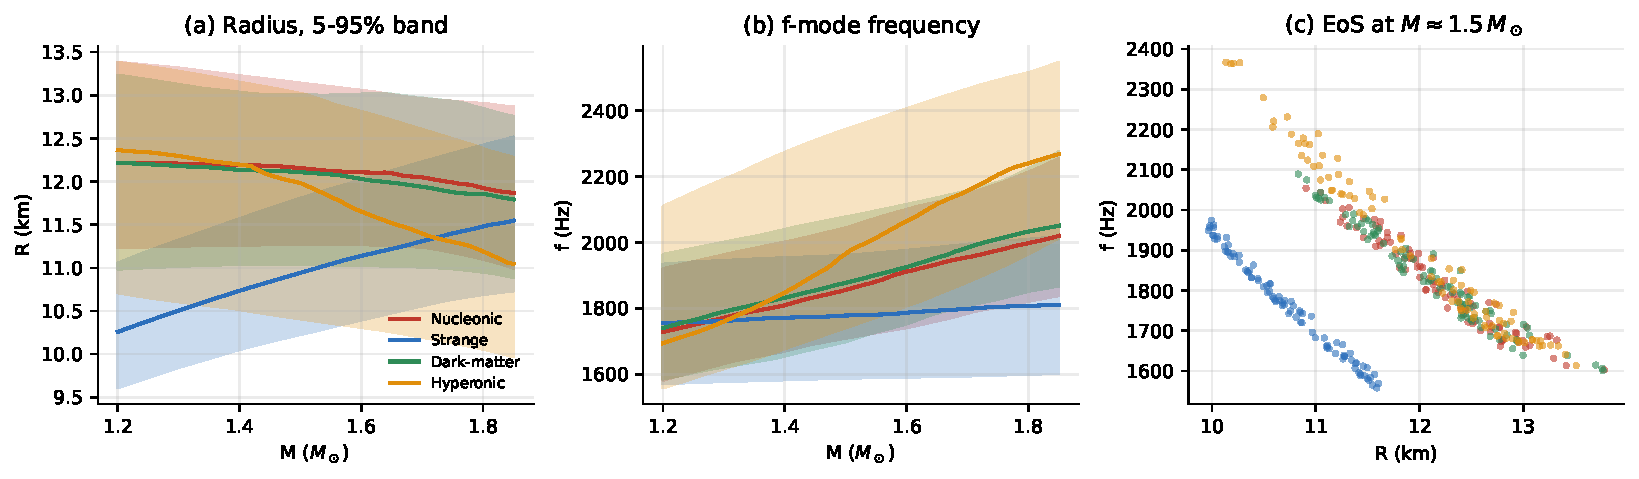
\includegraphics[width=\textwidth]{figs/figP1_population.pdf}
\caption{Population data set. (a) Radius and (b) $f$-mode frequency versus mass; lines are medians and bands the 5--95\% range across EoS of each scenario. (c) $f$ versus $R$ at $1.5\,\Msun$, one point per EoS.}\label{fig:pop}\end{figure}

\section{Methods}\label{sec:methods}
\subsection{Whole-EoS validation}
Every EoS belongs to exactly one of five folds (stratified by scenario). In each of five rounds one fold is the test set, the next fold is the calibration set and the other three are the training set; no EoS appears in more than one role, so every reported number is for EoS the classifier has never seen. The partition is repeated for three random seeds; we report the mean over folds within a repetition and Student-$t$ 95\% intervals over the three repetitions. Observations are $(M,R,f,\tau)$ at masses drawn uniformly over $1.2$--$1.85\,\Msun$ (a mass prior shared by all classes), with independent noise draws, and classes are balanced (chance 25\%). Accuracy is the fraction of correctly classified stars. The \emph{pair accuracy} between the nucleonic and dark-matter classes is the fraction of correct labels among those test stars of these two classes that the four-class classifier assigns to one of them (chance 50\%); it isolates the nucleonic--dark-matter confusion from the confusion with the other classes. Stars are drawn on a grid of 33 masses per EoS within the window.

\subsection{Observational-error scenarios}\label{sec:errors}
Observables are perturbed multiplicatively, $x_j^{\rm obs}=x_j(1+\sigma_j\epsilon_j)$, $\epsilon_j\sim\mathcal N(0,1)$ independent. Draws with a non-positive factor (only possible for the damping time at large $s$: 0.6\% of the draws at $s=2$ and 11\% at $s=4$; none elsewhere) are redrawn, so the noise is a truncated Gaussian; the kernel-Bayes likelihood ignores this truncation.
\emph{Literature-anchored scenarios:}
\textbf{NICER-like}: $\sigma_M=10\%$, $\sigma_R=9\%$, no $f$ or $\tau$; these are the 68\% uncertainties of the NICER analyses of PSR J0030+0451 ($M=1.34^{+0.15}_{-0.16}$ and $1.44^{+0.15}_{-0.14}\,\Msun$, $R=12.71^{+1.14}_{-1.19}$ and $13.02^{+1.24}_{-1.06}$\,km; \citealt{Riley19,Miller19}).
\textbf{NICER-like plus $f$-mode}: in addition $\sigma_f=20\%$, motivated by the forecast that third-generation detectors could measure the $f$-mode frequency of a GW170817-like inspiral to within a few hundred Hz \citep{Williams22}, i.e.\ roughly 10--25\% of $f$. These two are illustrative combinations drawn from different sources (a NICER pulsar and a hypothetical GW170817-like inspiral), not a realistic joint observation: mass, radius and $f$-mode of a single object are not currently available together.
\emph{Precision scale:} to show what would be required, the same observables are also evaluated with errors $s\times(5\%,5\%,2\%,20\%)$ in $(M,R,f,\tau)$ for $s\in\{0.25,0.5,1,2,4\}$, and in the noise-free limit. These values are not forecasts for any instrument; they define a scale on which the literature-anchored scenarios can be placed. Three observable sets are used: $\{M,R\}$, $\{M,R,f\}$ and $\{M,R,f,\tau\}$.

\subsection{Classifiers}
Learners: logistic regression, $k$-nearest neighbours ($k=25$), a random forest (200 trees, minimum leaf 5), histogram gradient boosting, an RBF support-vector machine (8000 training samples) and an MLP deep ensemble \citep{Lakshminarayanan17} of three $2\times64$ ReLU networks on log-transformed, standardised inputs, with default or lightly tuned settings; the effect of tuning and of alternative features is tested in Sec.~\ref{sec:tuned}. Training data contain three noise realisations of 33 masses for each training EoS.

\subsection{Kernel-Bayes reference classifier}
For a reference set of $(\mathrm{EoS},M)$ points the posterior of class $k$ for an observation $\mathbf x^{\rm obs}$ is
\begin{equation}
P(k\mid\mathbf x^{\rm obs})\;\propto\;\frac1{N_k}\sum_{i\in k}\prod_j\mathcal N\!\left(x^{\rm obs}_j;\,x_{ij},\,(\sigma_jx_{ij})^2\right),
\end{equation}
which is the Bayes-optimal classifier for the stated error model and a uniform prior over the reference EoS and masses. We use the training EoS as reference (the same information as the learners) and, separately, all EoS except the test fold (a larger reference). Unlike the single-sequence oracle of Appendix~\ref{sec:legacynoise}, this is not an upper bound, because the test EoS are not in the reference set; agreement between learners and kernel-Bayes indicates that the remaining error is set by the information in the observables rather than by the learner.

\subsection{Uncertainty quantification}\label{sec:uncmethods}
\emph{Calibration}: expected calibration error (ECE, 15 bins), negative log-likelihood (NLL) and Brier score, before and after temperature scaling fitted on the calibration EoS. \emph{Epistemic uncertainty}: mutual information across ensemble members. \emph{Conformal prediction}: split conformal prediction with the score $1-\hat p(y\mid x)$ at target miscoverage $\alpha=0.1$ \citep{Vovk05,Angelopoulos23}, calibrated on the calibration EoS with \emph{one star per calibration EoS}: for each of the $n\approx72$ calibration EoS one star (random mass, one noise draw) is chosen, so that each calibration unit comes from a different EoS and, if the EoS are exchangeable draws from one population, is exchangeable with a test star drawn the same way from a new EoS. The score quantile is taken at level $\lceil(n+1)(1-\alpha)\rceil/n$, as in standard split conformal prediction, and the reported sets and coverage are averages over 40 random choices of the calibration stars. The textbook finite-sample guarantee requires the calibration and test units to be exchangeable. Here the folds are stratified and class-balanced: the calibration fold contains a fixed number of EoS per class, the test EoS come from a disjoint fold with the same composition, and both are drawn without replacement from a finite catalogue. Exchangeability then holds within each class and for the class-balanced mixture only approximately (conditioning on the fixed class counts of the calibration fold breaks it by an amount of order $1/n$), so we do not claim the exact distribution-free guarantee; the coverage reported is an \emph{empirical marginal coverage} for stars of unseen EoS drawn from the same catalogue distribution with a uniform class prior. As a sensitivity check, a pooled variant that uses all stars of the calibration EoS (33 masses, two noise draws each) with the same $n$ is also reported; its stars are correlated, so for it even the approximate exchangeability argument fails. The coverage is marginal, not conditional on class or mass, and assumes that the EoS of the catalogue are exchangeable draws from one population; it does not extend to EoS from another population (Sec.~\ref{sec:popB}).

\section{Results}\label{sec:results}
\subsection{Noise-free separability of EoS populations}
Figure~\ref{fig:nf} shows the held-out-EoS accuracy without measurement error, and the left panel of Fig.~\ref{fig:cmpop} the confusion matrix. With $M$ and $R$ only the accuracy is 39\% (MLP ensemble; logistic regression 36\%, random forest 39\%); adding the $f$-mode raises it to 65\% and adding $\tau$ changes nothing (65\%). All learners agree within a few points. The confusion matrix shows why the ceiling is so low: strange matter is recognised perfectly (100\%), hyperonic-like matter in 76\% of cases, but nucleonic and dark-matter-admixed stars are assigned to each other almost at random (recall 50\% and 33\%; accuracy between the two classes 51\%, chance 50\%). Merging them into one class gives 84\% three-class accuracy; the baseline for this merged problem is 50\% (always predicting the merged class, which holds half of the stars), not the 33\% of three balanced classes. The reason is physical: the dark component shifts $f$ by only 0.57\% at fixed nuclear EoS (median over the population; 25.7\,Hz or 1.3\% for SLy with $G=100$\,fm$^2$; Sec.~\ref{sec:paired}), far less than the spread of $f$ at fixed mass produced by the uncertain nuclear EoS (a relative standard deviation of 6.2\% among the nucleonic EoS at $1.4\,\Msun$, and a full range of about $\pm12\%$ in Table~\ref{tab:popdata}).
\begin{figure}[t]\centering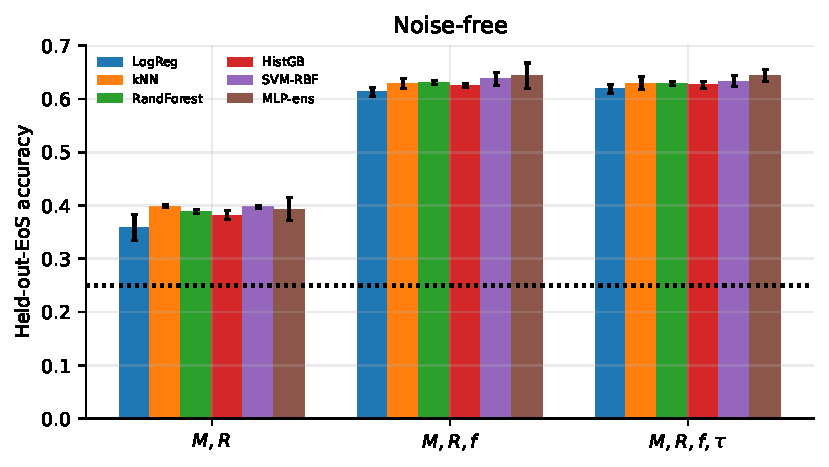
\includegraphics[width=.75\textwidth]{figs/figP2_noisefree.pdf}
\caption{Held-out-EoS accuracy without measurement error for each learner and observable set (95\% $t$-intervals over three repetitions; dotted: chance).}\label{fig:nf}\end{figure}

\subsection{Errors anchored on published measurements}\label{sec:anchored}
Table~\ref{tab:scen} gives the accuracy under the literature-anchored scenarios and at selected points of the precision scale. With NICER-like errors ($M$ 10\%, $R$ 9\%) the accuracy is 33\% (MLP ensemble; kernel-Bayes 34\%), barely above the 25\% chance level; adding a 20\% $f$-mode measurement raises it to 37\%. The three-class accuracy after merging nucleonic and dark-matter-admixed matter is 51\%, no better than the 50\% majority-class baseline of the merged problem. Errors of 5\%, 5\% and 2\% in $(M,R,f)$ would give 53\%, and 1.3\%, 1.3\%, 0.5\% would give 61\%, which approaches but never exceeds the noise-free ceiling of 65\%.
\begin{table}[t]\centering\small
\caption{Held-out-EoS accuracy (\%, mean $\pm$ 95\% $t$-interval over three repetitions) by error scenario and learner. Chance is 25\%.}\label{tab:scen}
\begin{tabular}{lccccccc}\toprule
Scenario & LogReg & $k$-NN & RF & HistGB & SVM & MLP ens. & Kernel Bayes\\\midrule
NICER-like: $M,R$ at 10\%, 9\% & 33$\pm$1 & 32$\pm$1 & 31$\pm$1 & 33$\pm$1 & 33$\pm$1 & 34$\pm$1 & 34$\pm$1 \\
+ $f$-mode at 20\% & 36$\pm$1 & 35$\pm$0 & 36$\pm$1 & 37$\pm$1 & 37$\pm$0 & 37$\pm$0 & 37$\pm$1 \\
$s=1$: 5\%, 5\%, 2\% & 51$\pm$1 & 52$\pm$1 & 53$\pm$1 & 53$\pm$2 & 53$\pm$2 & 53$\pm$1 & 53$\pm$2 \\
$s=1$ with $\tau$ 20\% & 51$\pm$1 & 52$\pm$0 & 52$\pm$1 & 53$\pm$1 & 53$\pm$2 & 53$\pm$1 & 53$\pm$2 \\
$s=0.25$ (1.3\%, 1.3\%, 0.5\%, 5\%) & 59$\pm$0 & 60$\pm$1 & 60$\pm$1 & 60$\pm$2 & 60$\pm$2 & 61$\pm$2 & 60$\pm$2\\\bottomrule\end{tabular}\end{table}

\subsection{Precision scale and which observable matters}
Figure~\ref{fig:dial} shows the accuracy against the precision scale. For the MLP ensemble, $\{M,R\}$ gives 38\%, 37\% and 30\% at $s=0.25$, 1 and 4, whereas $\{M,R,f\}$ gives 61\%, 53\% and 38\%; the damping time with a 20\% error (scaled with $s$) adds nothing within the uncertainty. Learners and kernel-Bayes agree to a few points at every scale (at $s=1$: MLP 53\%, kernel-Bayes 53\%, kernel-Bayes with all other EoS as reference 53\%; logistic regression 50\%, random forest 52\%, gradient boosting 52\%, SVM 52\%), so none of the learners tried leaves a measurable amount of information unused, and enlarging the reference sample from the training EoS to all other EoS does not change the result (this is evidence for an information plateau within these priors, not a proof of an upper bound).
\begin{figure}[t]\centering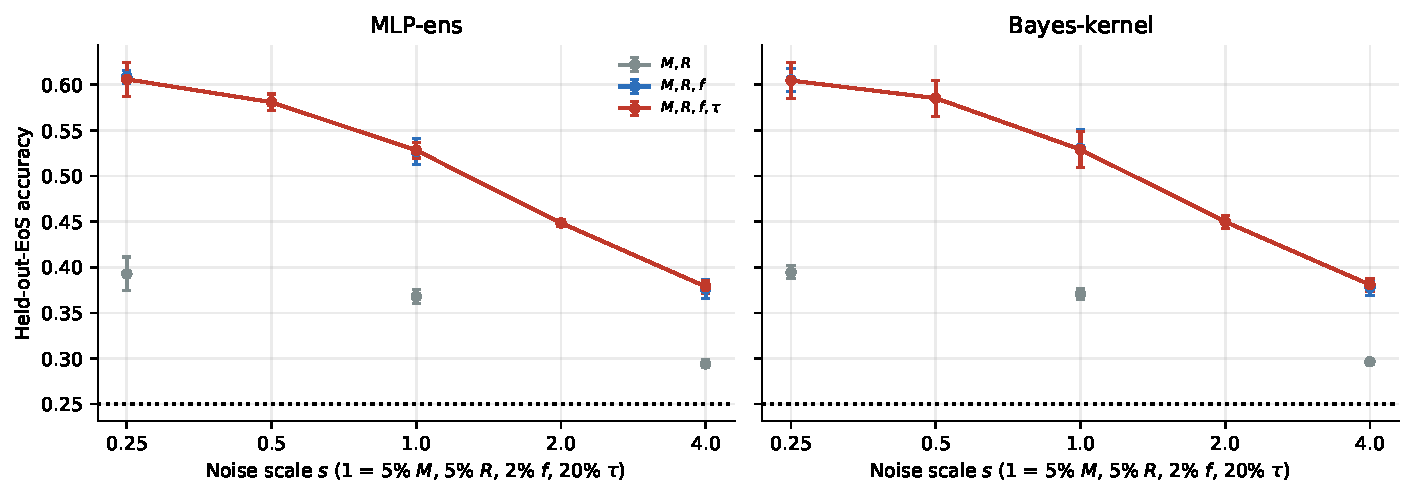
\includegraphics[width=\textwidth]{figs/figP3_dial.pdf}
\caption{Held-out-EoS accuracy versus precision scale $s$ (1 = 5\%, 5\%, 2\%, 20\% in $M,R,f,\tau$) for the MLP ensemble and the kernel-Bayes classifier, for three observable sets (95\% $t$-intervals; dotted: chance). The $\{M,R,f\}$ and $\{M,R,f,\tau\}$ curves coincide.}\label{fig:dial}\end{figure}

\subsection{Degeneracies}
Figure~\ref{fig:cmpop} shows row-normalised confusion matrices. With accurate $f$ ($s=0.25$) strange matter is still identified perfectly (100\%) and the hyperonic-like class in 63\%, but the nucleonic and dark-matter rows remain mixed (48\% and 31\% correct, 33\% and 49\% assigned to each other). With a 20\% $f$-mode error all rows are confused with all columns, strange matter being the best recovered (66\%).
\paragraph{Is any subset of the nucleonic and dark-matter stars separable?} The confusion does not seem to be confined to particular stars. A two-class classifier trained on nucleonic and dark-matter EoS only (noise-free; whole-EoS five-fold cross-validation, 10 repetitions) has a balanced accuracy of 52\% (random forest) and 51\% (gradient boosting) overall; 50, 50 and 54\% (random forest) when the test stars are restricted to the mass bins $1.2$--$1.4$, $1.4$--$1.6$ and $1.6$--$1.85\,\Msun$; and 52, 53 and 50\% when the dark-matter test EoS are restricted to the lowest, middle and highest tercile of the self-interaction strength $G$ (the lowest tercile, $G\le189$\,fm$^2$, has the largest shifts; the dark component is expected to matter more for heavier stars, whose median shift is larger, Sec.~\ref{sec:paired}). All random-forest and gradient-boosting values lie between 48 and 54\%. The EoS-level sampling error of each value is about 4--6 points (the spread over repetitions, below 1.6 points, understates it because the same EoS are reused), so these values are compatible with chance; logistic regression is at or slightly below 50\%.
\begin{figure}[t]\centering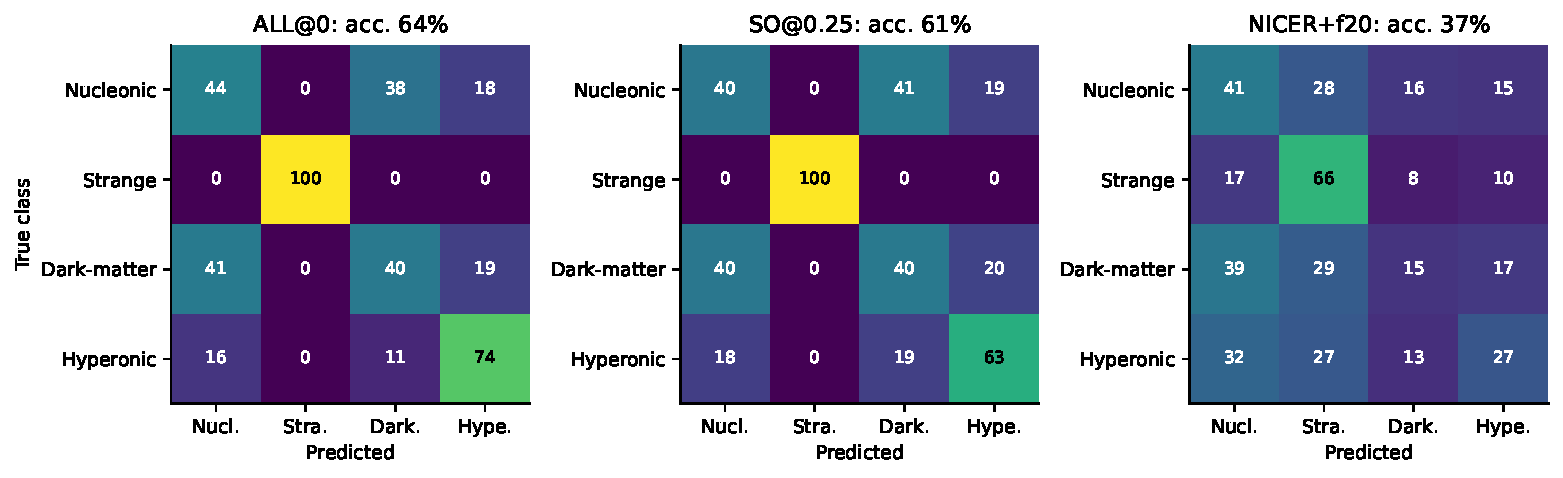
\includegraphics[width=\textwidth]{figs/figP4_confusion.pdf}
\caption{Row-normalised confusion matrices (\%) of the temperature-scaled MLP ensemble, pooled over folds and repetitions. Left to right: noise-free, $s=0.25$, and NICER-like errors plus a 20\% $f$-mode measurement.}\label{fig:cmpop}\end{figure}

\subsection{Does tuning or feature engineering break the plateau?}\label{sec:tuned}
A natural objection is that the plateau reflects untuned learners or uninformative features. Each of the six learners was therefore given a small hyper-parameter grid (Appendix~\ref{sec:settings}); the configuration with the highest accuracy on the calibration EoS was applied to the test EoS (``selected''), and the highest test accuracy over the grid (``best on test'', optimistic because it is chosen on the test fold) is given in brackets. Two feature sets were compared: $\ln(M,R,f,\tau)$, and engineered features $(\ln M,\ln R,\ln[f/\sqrt{M/R^3}],\ln[\tau M^3/R^4])$ that remove the leading Newtonian scalings of the $f$-mode and damping time. Table~\ref{tab:tuned} shows that tuning moves the noise-free accuracy by at most a few points, from 60--64\% to at best 66\% on the test fold, that the engineered features do not help (at best 66\%), and that the same holds at $s=0.25$ (at best 62\% and 61\%). The mean nucleonic--dark-matter pair accuracy over the six learners stays at 51\% (noise-free) and 49\% ($s=0.25$). Neither tuning nor feature engineering therefore changes the picture, which supports the view that the limit is set by the overlap of the populations rather than by the learner; the grids are finite, and a different search could in principle do better.
\begin{table}[t]\centering\small
\caption{Held-out-EoS accuracy (\%) of tuned learners: configuration selected on the calibration EoS (best accuracy over the grid on the test fold in brackets), for raw and engineered features; mean over 2 repetitions of 5 folds. Chance is 25\%.}\label{tab:tuned}
\begin{tabular}{llcccccc}\toprule
Errors & Features & LogReg & $k$-NN & RF & HistGB & SVM & MLP\\\midrulenoise-free & raw & 60 (60) & 61 (62) & 62 (63) & 62 (64) & 64 (66) & 64 (66) \\
noise-free & engineered & 60 (60) & 63 (65) & 63 (64) & 64 (65) & 65 (66) & 64 (65) \\
$s=$0.25 & raw & 57 (57) & 59 (60) & 59 (60) & 60 (61) & 59 (61) & 60 (62) \\
$s=$0.25 & engineered & 57 (57) & 60 (60) & 60 (60) & 60 (61) & 60 (61) & 60 (61)\\\bottomrule\end{tabular}\end{table}

\subsection{Dark matter when the nuclear EoS is known}\label{sec:paired}
To separate ``the dark component is small'' from ``the nuclear EoS is unknown'', the observables of each of the 90 dark-matter-admixed EoS were also computed for its own nuclear base EoS without the dark component, at the same masses. At fixed nuclear EoS and mass the dark component raises $f$ by a median of 0.57\% (EoS-level bootstrap interval of the median 0.50--0.66\%, conditional on the construction below; 5--95\% range 0.27--2.22\%; positive for 100\% of the pairs) and lowers $R$ by a median of -0.40\% (-1.50 to -0.20\%); the median shift grows mildly with mass, from 0.43\% at $1.2\,\Msun$ to 0.50, 0.57 and 0.71\% at 1.4, 1.6 and $1.8\,\Msun$ (radius: -0.31 to -0.51\%); the shift falls steeply with the self-interaction (Fig.~\ref{fig:paired}a; correlation of $\ln G$ with $\Delta f/f$ at $1.4\,\Msun$ is -0.95). \emph{The shift is not independent of the model construction:} when the baryon-number normalisation of the one-fluid barotrope is changed to its extreme value, the shift of an individual EoS changes by a median of 5\% and at most 6\% (and by up to 65\% for EoS with $m_\chi$ above the stability window in the wide-prior sample; see the paragraph on the dark-matter construction below), and the bootstrap interval reflects the EoS sample, not this modelling uncertainty. If the observer were told the nuclear EoS exactly, the Bayes accuracy for dark matter versus no dark matter (equal priors, independent Gaussian errors, mass identical by construction) would reach 75\% at $\sigma_f=0.51\%$ (EoS-level bootstrap interval 0.45--0.59\%) when $R$ is known to 1\% (0.51\% for 5\%) and 90\% at $\sigma_f=0.20\%$ (0.17--0.23\%) (Fig.~\ref{fig:paired}b); at the points of the precision scale it is 76\% at $s=0.25$ (0.5\% in $f$, 1.25\% in $R$), 58\% at $s=1$ and 52\% at $s=4$, and with a 20\% $f$-mode error and 9\% in $R$ it is 52\%. With the nuclear EoS \emph{unknown} the accuracy between the nucleonic and dark-matter classes is 51\% even without any measurement error (Sec.~\ref{sec:results}). The lack of discrimination therefore comes from the uncertainty of the nuclear EoS, not from the smallness of the shift alone: detecting the dark component needs both an $f$-mode measurement at the 0.5\% level and a nuclear EoS known to better than the shift itself.
\paragraph{Sensitivity to the dark-matter construction.} The one-fluid barotrope assigns baryon number through $n_B=\rho/m_0$. This paper uses $m_0=931.494$\,MeV (the atomic mass unit, the normalisation of the polytropic fits); the companion pilot \citep{HusainPilot} uses $m_0=931.192$\,MeV. The baryon chemical potential $\mu_N\to m_0$ at low density, so $m_0$ fixes where $\mu_N$ exceeds $m_\chi$ and the dark component appears, and it is not a free parameter of the dark-matter physics but a convention of the effective barotrope. The two values give the same shift to within 0.2\% for a typical EoS (at most 0.2\% over the 90 EoS tested; for SLy with $G=100$\,fm$^2$, 25.7\,Hz here against 25.8\,Hz in the pilot, a difference that also includes the different solvers), so the reconciliation of the two normalisations does not matter at the level of the headline number. Larger changes of convention move the population median very little: with $m_0=935$ and $938.9$\,MeV (the latter places the threshold at zero density) the median shifts at $1.4\,\Msun$ are 0.51\% and 0.51\% against 0.50\% (5--95\% ranges 0.27--2.04 and 0.28--2.09\% against 0.26--1.99\%), but for an individual EoS of the primary (in-window) population the shift changes by a median of 5\% and at most 6\% between the default and the extreme prescription. The sensitivity is much larger when $m_\chi$ lies above the stability window: for the 7 EoS of the earlier wide-prior sample with $m_\chi>938.783$\,MeV (of 16 tested) the change has a median of 9\% and a maximum of 65\%, the largest changes (23--65\%) occurring for three EoS with $m_\chi=939.00$--939.03\,MeV, just above the extreme normalisation of 938.9\,MeV; the in-window EoS of that sample change by at most 6\%. The shift depends much more on $G$ (correlation of $\ln G$ with $\Delta f/f$: -0.95) than on $m_\chi$ (correlation -0.04). The qualitative conclusion is unchanged, but the shift of a single EoS depends on the prescription at the per-cent level inside the window (and strongly outside it), so the quantitative detectability thresholds above (e.g.\ the $f$-mode precision for 75\% accuracy) carry this modelling uncertainty in addition to their statistical intervals, and the effective one-fluid oscillation model (equilibrium composition, common displacement of the two components) remains an explicit assumption of every dark-matter statement in this paper.
\begin{figure}[t]\centering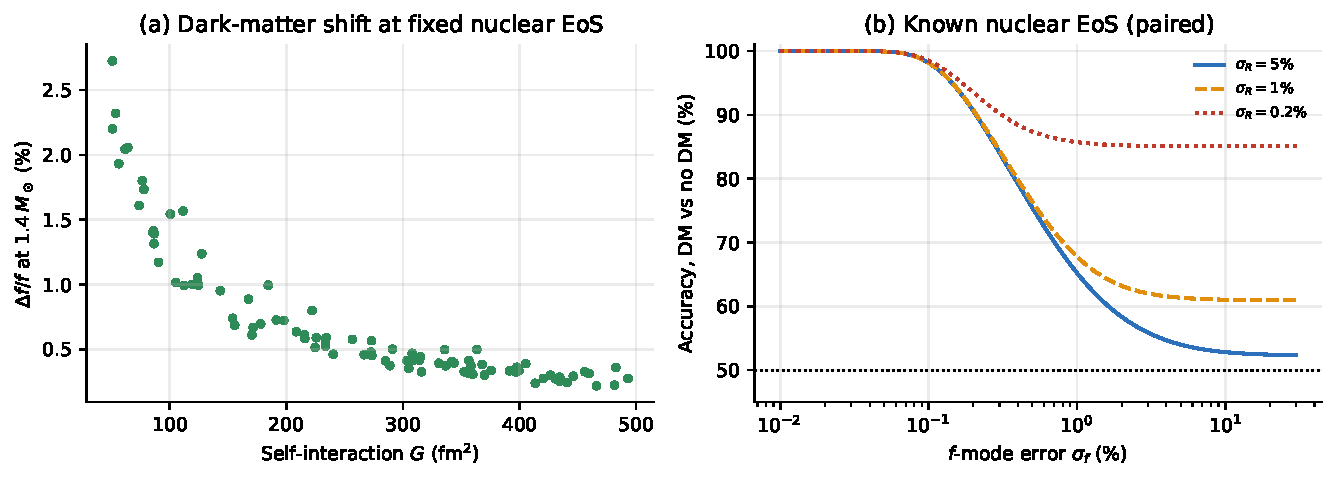
\includegraphics[width=.95\textwidth]{figs/figP6_paired.pdf}
\caption{Dark matter at fixed nuclear EoS (90 paired EoS). (a) Fractional $f$-mode shift at $1.4\,\Msun$ versus the self-interaction $G$. (b) Bayes accuracy for dark matter versus no dark matter, averaged over EoS and masses, as a function of the $f$-mode error for three radius errors (dotted: chance).}\label{fig:paired}\end{figure}

\subsection{How well must the nuclear EoS be known?}\label{sec:narrow}
The population results above correspond to the wide nuclear prior of Table~\ref{tab:priors}, and the paired results to an exactly known nuclear EoS. To connect the two, nucleonic and dark-matter populations were generated with the four polytropic parameters confined to windows about the SLy fit \citep{Read09}, whose half-widths are the fraction $w$ of the half-widths of the main prior ($w=0.4$, 0.2, 0.1, 0.05 and 0.02; for $w=0.02$ the half-widths are $\pm0.0045$\,dex in $\log_{10}P_1$ and $\pm0.014$--0.017 in the $\Gamma_i$). The same restriction applies to both classes, the dark-sector prior is unchanged, and the solver and screens are those of the main population; there are 40 EoS per class and window with five masses each ($1.2$--$1.9\,\Msun$). Table~\ref{tab:narrow} and Fig.~\ref{fig:narrow} give, for each window, the spread $\sigma_f$ of $f$ at $1.4\,\Msun$ among the nucleonic EoS and the balanced nucleonic--dark-matter accuracy of three learners.

The spread falls from 6.2\% for the main prior to 3.1, 1.9, 1.2, 0.6 and 0.2\% for the five windows. Without measurement error the accuracy stays between 51 and 58\% as long as $\sigma_f\gtrsim1\%$, rises to 62--65\% when $\sigma_f$ (0.6\%) is comparable to the median dark-matter shift (0.57\%), and reaches 81\% at $\sigma_f=0.2\%$. Measurement error limits the gain: with an $f$-mode error of 0.5\% ($s=0.25$) the best accuracy is 62--64\% at the narrowest window, and with 2\% ($s=1$) it never exceeds 55\%. With 40 EoS per class the EoS-level binomial standard error of each value is about 5--6 points, so the rise to 81\% is significant while the values near 62\% are only about two standard errors above chance. Detecting the dark component therefore needs \emph{both} the spread of $f$ among the allowed nuclear EoS \emph{and} the $f$-mode measurement error to be at or below the size of the shift, in line with the paired result (Sec.~\ref{sec:paired}). The windows are centred on a single fiducial EoS, confine only the polytropic parameters (the crust is fixed), and ignore the correlations between parameters that a real constraint would have, so $w$ is not a statement about any actual constraint on the nuclear EoS.
\begin{table}[t]\centering\small
\caption{Nucleonic versus dark-matter balanced accuracy (\%) as the nuclear parameters are confined to windows of fractional half-width $w$ about the SLy fit. $\sigma_f$: relative spread of $f$ at $1.4\,\Msun$ among the nucleonic EoS. LR: logistic regression, RF: random forest, GB: gradient boosting; whole-EoS five-fold cross-validation, 10 repetitions; chance 50\%.}\label{tab:narrow}
\begin{tabular}{lccccccccccc}\toprule
 & & & \multicolumn{3}{c}{noise-free} & \multicolumn{3}{c}{$s=0.25$} & \multicolumn{3}{c}{$s=1$}\\\cmidrule(lr){4-6}\cmidrule(lr){7-9}\cmidrule(lr){10-12}
$w$ & $N$ per class & $\sigma_f$ (\%) & LR & RF & GB & LR & RF & GB & LR & RF & GB\\\midrule0.4 & 40 & 3.1 & 55 & 51 & 51 & 56 & 51 & 51 & 55 & 51 & 52 \\
0.2 & 40 & 1.9 & 54 & 55 & 55 & 54 & 50 & 50 & 53 & 50 & 50 \\
0.1 & 40 & 1.2 & 58 & 52 & 53 & 58 & 53 & 53 & 54 & 51 & 51 \\
0.05 & 40 & 0.6 & 65 & 62 & 62 & 61 & 59 & 60 & 55 & 52 & 52 \\
0.02 & 40 & 0.2 & 80 & 81 & 81 & 64 & 62 & 63 & 55 & 52 & 53\\\bottomrule\end{tabular}\end{table}
\begin{figure}[t]\centering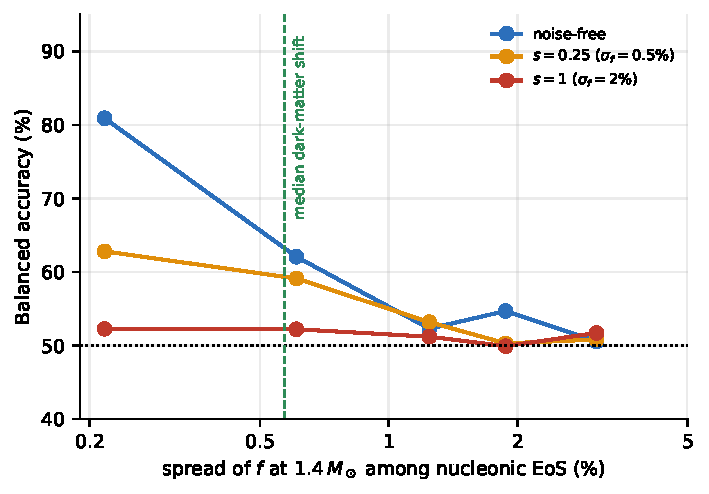
\includegraphics[width=.62\textwidth]{figs/figP8_narrow.pdf}
\caption{Balanced nucleonic-versus-dark-matter accuracy (mean of random forest and gradient boosting) against the spread of $f$ at $1.4\,\Msun$ among nucleonic EoS, for nuclear parameters confined to windows about the SLy fit (Table~\ref{tab:narrow}). Dotted: chance; dashed: median dark-matter shift.}\label{fig:narrow}\end{figure}
\paragraph{Subsets of the main population.} As a first, coarse test the main population was restricted to EoS whose four polytropic parameters all lie in the central fraction $w$ of their prior ranges (the same restriction for both classes; Table~\ref{tab:pw}). For $w=1$, 0.9, 0.8 and 0.7 (down to 32 nucleonic and 23 dark-matter EoS) the accuracy of logistic regression and of a random forest stays between 45\% and 61\% in the noise-free case and at $s=0.25$ and $s=1$. The highest value (61\%, random forest, noise-free, $w=0.7$) rests on 55 EoS, for which the binomial standard error is about 7 points, and it is not accompanied by a rise in the other settings or for logistic regression, so the values are compatible with chance at these sample sizes; narrowing the prior by 30\% per parameter does not make the dark component recognisable in these experiments. Substantially narrower priors would leave too few EoS in this catalogue, The finer windows above, and the limit of an exactly known nuclear EoS (Sec.~\ref{sec:paired}), probe much narrower priors.
\begin{table}[t]\centering\small
\caption{Accuracy (\%) between the nucleonic and dark-matter classes versus the central fraction $w$ of the nuclear parameter ranges (10 repetitions of 5-fold whole-EoS cross-validation; chance 50\%). $N$ is the number of nucleonic + dark-matter EoS.}\label{tab:pw}
\begin{tabular}{llcrr}\toprule
Errors & $w$ & $N$ & LogReg & RF\\\midrulenoise-free & 1 & 90+90 & 47 & 51 \\
noise-free & 0.9 & 58+63 & 45 & 50 \\
noise-free & 0.8 & 47+37 & 55 & 50 \\
noise-free & 0.7 & 32+24 & 53 & 56 \\
$s=$0.25 & 1 & 90+90 & 48 & 49 \\
$s=$0.25 & 0.9 & 58+63 & 49 & 49 \\
$s=$0.25 & 0.8 & 47+37 & 52 & 48 \\
$s=$0.25 & 0.7 & 32+24 & 50 & 50 \\
$s=$1 & 1 & 90+90 & 49 & 49 \\
$s=$1 & 0.9 & 58+63 & 46 & 48 \\
$s=$1 & 0.8 & 47+37 & 50 & 49 \\
$s=$1 & 0.7 & 32+24 & 53 & 49\\\bottomrule\end{tabular}\end{table}
\subsection{Calibration and prediction sets}\label{sec:unc}
The probabilities are well calibrated because the learners are close to the information limit (Fig.~\ref{fig:uncpop}a): at $s=1$ the ECE is 0.041 for the raw ensemble, 0.040 after temperature scaling and 0.041 for kernel-Bayes, with NLL 0.92 nats for all three (Table~\ref{tab:uncpop}). Conformal sets calibrated with one star per EoS have empirical marginal coverage of 0.91--0.92 at the 0.90 target for every scenario (as expected for the finite-sample-corrected quantile; no formal guarantee is claimed for the stratified folds, Sec.~\ref{sec:uncmethods}); the pooled variant gives 0.91--0.92 with almost identical sets (2.24 against 2.25 at $s=1$). The price of validity is set size: 3.32 of four classes under NICER-like errors, 3.22 when a 20\% $f$-mode is added, 2.25 at $s=1$ and 1.87 at $s=0.25$. Temperature scaling and kernel-Bayes give the same sets. At realistic precision the data therefore support a short list containing most of the classes, not a single label.
\begin{table}[t]\centering\small
\caption{Calibration and conformal sets (mean over three repetitions): ECE and NLL (nats) for the raw MLP ensemble, the temperature-scaled ensemble ($+T$) and kernel-Bayes, and coverage and set size (target coverage 0.90) of the conformal sets calibrated with one star per EoS.}\label{tab:uncpop}
\begin{tabular}{lccccccrrrr}\toprule
 & \multicolumn{3}{c}{ECE} & \multicolumn{3}{c}{NLL} & \multicolumn{2}{c}{MLP $+T$} & \multicolumn{2}{c}{Kernel Bayes}\\\cmidrule(lr){2-4}\cmidrule(lr){5-7}\cmidrule(lr){8-9}\cmidrule(lr){10-11}
Scenario & Raw & $+T$ & KB & Raw & $+T$ & KB & Cov. & Size & Cov. & Size\\\midruleNICER-like & 0.021 & 0.023 & 0.019 & 1.32 & 1.32 & 1.32 & 0.92 & 3.32 & 0.92 & 3.31 \\
+ $f$ at 20\% & 0.021 & 0.022 & 0.020 & 1.29 & 1.29 & 1.29 & 0.92 & 3.23 & 0.92 & 3.23 \\
$s=0.25$ & 0.053 & 0.043 & 0.093 & 0.71 & 0.71 & 0.83 & 0.92 & 1.87 & 0.92 & 1.94 \\
$s=0.5$ & 0.043 & 0.039 & 0.054 & 0.75 & 0.75 & 0.77 & 0.91 & 1.95 & 0.92 & 1.99 \\
$s=1$ & 0.038 & 0.037 & 0.039 & 0.92 & 0.92 & 0.92 & 0.92 & 2.26 & 0.92 & 2.27 \\
$s=2$ & 0.031 & 0.033 & 0.026 & 1.15 & 1.15 & 1.15 & 0.92 & 2.88 & 0.92 & 2.86 \\
$s=4$ & 0.026 & 0.028 & 0.021 & 1.29 & 1.29 & 1.29 & 0.92 & 3.27 & 0.92 & 3.25\\\bottomrule\end{tabular}\end{table}
\begin{figure}[t]\centering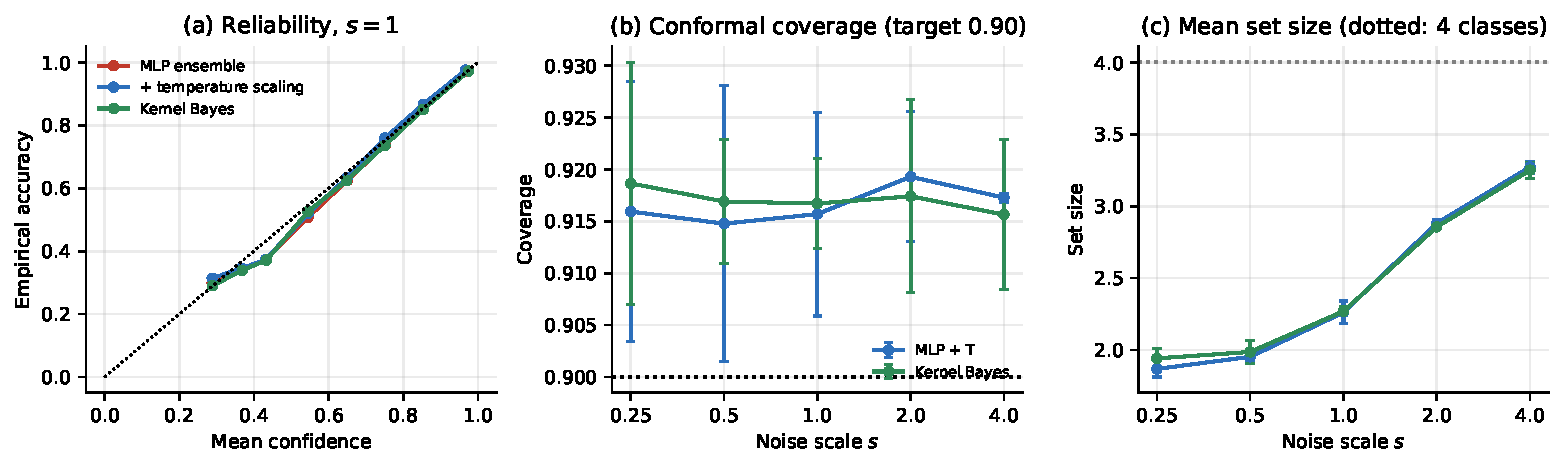
\includegraphics[width=\textwidth]{figs/figP5_uncertainty.pdf}
\caption{(a) Reliability diagram ($s=1$, pooled). (b) Conformal coverage and (c) mean prediction-set size versus precision scale (95\% $t$-intervals).}\label{fig:uncpop}\end{figure}

\subsection{Statistical robustness}\label{sec:robust}
\paragraph{EoS-level bootstrap.} The intervals of the preceding sections describe re-partitioning of the same 360 EoS. Table~\ref{tab:boot} instead gives 95\% intervals from resampling whole EoS within each class (2000 resamples; each EoS's predictions pooled over the three partitions). These intervals are \emph{conditional} on the catalogue and the trained classifiers: they quantify which EoS happen to be in the test sets, but not the variability from regenerating the EoS populations from the priors, from retraining the classifiers on a different catalogue, or from changing the priors themselves (the last two are only partly probed by the learning curves and by population~B). The noise-free accuracy of the MLP ensemble is 64\% [61, 67], the recall of strange matter is 100\% [100, 100], and the accuracy between the nucleonic and dark-matter classes is 51\% [45, 56]; with NICER-like errors and a 20\% $f$-mode it is 50\% [47, 52] and the overall accuracy 37\% [36, 38]. The intervals for the nucleonic--dark-matter pair contain 50\% in every scenario, so the absence of demonstrated discrimination is not an artefact of a particular partition of this finite sample; it remains conditional on the catalogue and priors, and an interval containing 50\% does not prove that the classes are identical, only that these experiments do not show a difference.
\begin{table}[t]\centering\small
\caption{EoS-level bootstrap estimates (\%, 95\% interval): overall accuracy, accuracy between the nucleonic and dark-matter classes (chance 50\%) and recall of strange matter.}\label{tab:boot}
\begin{tabular}{llccc}\toprule
Scenario & Learner & Accuracy & Nucleonic vs DM & Strange recall\\\midruleALL 0 & MLP-ens & 64 [61, 67] & 51 [45, 56] & 100 [100, 100] \\
ALL 0 & LogReg & 62 [59, 65] & 50 [44, 56] & 100 [100, 100] \\
ALL 0 & RandForest & 63 [60, 65] & 53 [49, 58] & 100 [100, 100] \\
NICER+f20 & MLP-ens & 37 [36, 38] & 50 [48, 53] & 67 [65, 68] \\
NICER+f20 & LogReg & 36 [34, 37] & 50 [47, 54] & 61 [59, 62] \\
NICER+f20 & RandForest & 35 [35, 36] & 50 [49, 51] & 58 [57, 60] \\
NICER+f20 & Bayes-kernel & 37 [36, 39] & 51 [48, 53] & 67 [65, 68] \\
SO 1.0 & MLP-ens & 53 [51, 55] & 49 [46, 52] & 91 [89, 92] \\
SO 1.0 & LogReg & 51 [48, 53] & 49 [45, 54] & 90 [89, 91] \\
SO 1.0 & RandForest & 53 [51, 54] & 50 [48, 51] & 89 [88, 90] \\
SO 1.0 & Bayes-kernel & 53 [51, 55] & 49 [46, 52] & 91 [89, 92] \\
SO 0.25 & MLP-ens & 60 [58, 63] & 49 [45, 54] & 100 [100, 100] \\
SO 0.25 & LogReg & 58 [56, 61] & 49 [44, 55] & 100 [100, 100] \\
SO 0.25 & RandForest & 60 [58, 62] & 50 [47, 53] & 100 [100, 100] \\
SO 0.25 & Bayes-kernel & 61 [58, 63] & 51 [48, 55] & 100 [100, 100]\\\bottomrule\end{tabular}\end{table}
\paragraph{Population size.} Figure~\ref{fig:lc} shows the accuracy as a function of the number of training EoS (54 to 216). Without noise the logistic regression is already at 62\% with 54 training EoS and the MLP ensemble at 62\% with 108, against 64\% with 216; under NICER-like errors plus a 20\% $f$-mode the accuracy is 35--37\% at every size. The plateau therefore does not appear to result from too few EoS, and a larger population of the same kind is unlikely to change the numbers.
\begin{figure}[t]\centering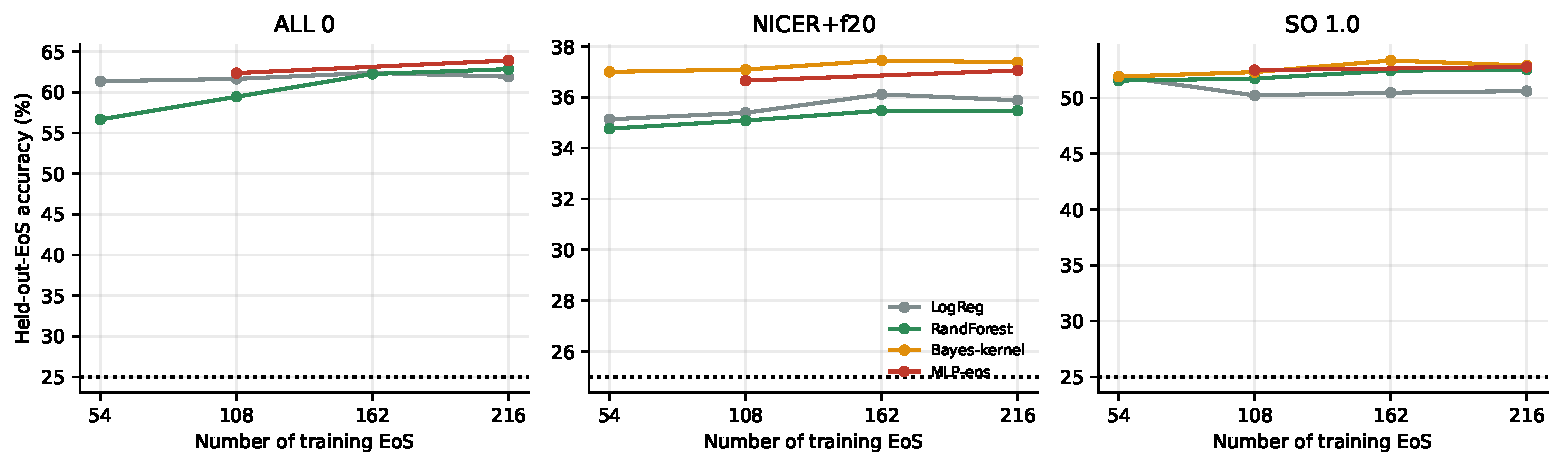
\includegraphics[width=\textwidth]{figs/figP7_learning.pdf}
\caption{Held-out-EoS accuracy versus the number of training EoS for four learners (pooled over repetitions; dotted: chance). The MLP ensemble is shown at 108 and 216 training EoS only.}\label{fig:lc}\end{figure}
\paragraph{Wider dark-fermion mass prior (sensitivity).} The primary population restricts $m_\chi$ to the stability window $937.9\le m_\chi\le938.783$\,MeV. As a sensitivity experiment the earlier population, whose dark-matter EoS drew $m_\chi$ up to 939.2\,MeV (27 of its 90 dark-matter EoS above the upper bound and 63 inside), was analysed with the same protocol; the other three classes are identical. The results are essentially the same as for the primary population: 64\% without noise, 61\% at $s=0.25$, 53\% at $s=1$ and 37\% for NICER-like errors plus a 20\% $f$-mode (MLP ensemble), with an accuracy of 52\% between the nucleonic and dark-matter classes (primary: 65\%, 61\%, 53\%, 37\% and 51\%).

\subsection{Robustness to the EoS populations}\label{sec:popB}
The preceding results depend on the parametrisations and priors of Table~\ref{tab:priors}. To test this, an alternative population (``B'') was constructed with different functional forms and priors (Table~\ref{tab:priorsB}); the same screens, solver and experiments were applied (48 EoS per scenario, 192 in total; Table~\ref{tab:popBdata}). Population~B is still parametric rather than microphysical, so it tests sensitivity to the parametrisation, not to the underlying nuclear physics.
\begin{table}[t]\centering\small
\caption{Alternative population B. $\varepsilon_x$ is the energy density at $1.3\,n_{\rm sat}$ ($\rho_x=10^{14.55}$\,g\,cm$^{-3}$); sound-speed profiles are piecewise linear in $\ln\varepsilon$ through knots at $\varepsilon/\varepsilon_x=1,1.5,2.5,4,7$ and constant above; the lower-density EoS is a single polytrope on the same crust.}\label{tab:priorsB}
\begin{tabular}{>{\raggedright\arraybackslash}p{.17\textwidth}p{.75\textwidth}}\toprule
Scenario & Parameters (uniform priors)\\\midrule
Nucleonic & polytrope $\log_{10}P_1\in[34.15,34.55]$, $\Gamma_1\in[2.6,3.6]$ up to $\rho_x$; then $c_s^2\in[0.1,1]$ at each knot (first knot $[0.1,0.6]$)\\
Hyperonic-like & as nucleonic, but $c_s^2\in[0.15,0.6]$ at the first two knots, a dip $c_s^2\in[0.03,0.3]$ at $2.5\,\varepsilon_x$ and $c_s^2\in[0.5,1]$ at the last two\\
Strange (self-bound) & $P(\mu)=3a_4\mu^4/(4\pi^2)-3a_2\mu^2/(4\pi^2)-B$ with $a_4\in[0.55,1]$, $\sqrt{a_2}\in[0,150]$\,MeV, $B^{1/4}\in[135,165]$\,MeV\\
Dark-matter admixed & nucleonic B plus a dark Fermi gas with $m_\chi\in[937.9,938.78]$\,MeV (inside the stability window) and $G\in[50,500]$\,fm$^2$\\\bottomrule\end{tabular}\end{table}
\begin{table}[t]\centering\small
\caption{Population B (48 EoS per scenario): ranges of $M_{\max}$ ($\Msun$), $R_{1.4}$ (km), $\Lambda_{1.4}$ and $f$ at $1.4\,\Msun$ (Hz).}\label{tab:popBdata}
\begin{tabular}{lrrrrr}\toprule
Scenario & $N$ & $M_{\max}$ & $R_{1.4}$ & $\Lambda_{1.4}$ & $f_{1.4}$\\\midruleNucleonic & 48 & 2.04--3.05 & 11.5--13.5 & 309--795 & 1563--1913 \\
Strange & 48 & 1.97--2.20 & 10.9--11.7 & 441--761 & 1575--1776 \\
Dark-matter & 48 & 2.01--3.05 & 11.6--13.7 & 287--798 & 1557--1947 \\
Hyperonic & 48 & 2.02--2.51 & 11.9--13.5 & 290--797 & 1556--1942\\\bottomrule\end{tabular}\end{table}
\paragraph{Within population B.} With whole-EoS hold-out, the MLP ensemble reaches 49\% without noise (logistic regression 52\%, random forest 52\%), against 65\% for population~A. Strange matter is again recognised perfectly (100\%) and the accuracy between the nucleonic and dark-matter classes is again at the level of chance (51\%); nucleonic matter is recognised in 34\%, dark-matter in 37\% and hyperonic-like matter in only 26\% (76\% in population~A), so the separability of the hyperonic-like family, and with it the overall plateau, depends on how the family is built. At $s=0.25$ and $s=1$ the accuracies are 50\% and 45\% (A: 61\% and 53\%), and for NICER-like errors plus a 20\% $f$-mode 37\% (A: 37\%); there strange matter is recognised in 74\% of cases.
\paragraph{Out-of-family transfer.} Table~\ref{tab:cross} gives the accuracy of classifiers trained on all EoS of one population and tested on all EoS of the other. Without noise the transfer accuracy is 54\% (A$\to$B) and 54\% (B$\to$A) for the MLP ensemble, between the within-population values, and with NICER-like errors plus a 20\% $f$-mode 36\% and 33\%. Strange matter is still recognised in 100\% and 100\% of cases without noise, and the accuracy between the nucleonic and dark-matter classes remains 52\% and 53\%. The results that survive a change of population are therefore (i) the absence of demonstrated nucleonic--dark-matter discrimination, (ii) an accuracy of about 33--37\% under NICER-like errors, with or without a 20\% $f$-mode, and (iii) the identifiability of self-bound strange matter once $f$ is accurate; the 65\% plateau and the identifiability of the hyperonic-like family are specific to the construction of population~A.
\begin{table}[t]\centering\small
\caption{Out-of-family test: accuracy (\%, mean $\pm$ 95\% $t$-interval over three noise realisations) of classifiers trained on all EoS of one population and tested on all EoS of the other. Chance is 25\%.}\label{tab:cross}
\begin{tabular}{llccccc}\toprule
Train$\to$test & Scenario & LogReg & RF & HistGB & MLP ens. & Kernel Bayes\\\midruleA$\to$B & ALL 0 & 52$\pm$0 & 50$\pm$0 & 50$\pm$7 & 52$\pm$5 & -- \\
A$\to$B & NICER+f20 & 35$\pm$1 & 34$\pm$1 & 36$\pm$1 & 36$\pm$1 & 36$\pm$1 \\
A$\to$B & SO 1.0 & 42$\pm$0 & 38$\pm$2 & 39$\pm$1 & 39$\pm$1 & 39$\pm$0 \\
A$\to$B & SO 0.25 & 52$\pm$0 & 47$\pm$1 & 46$\pm$2 & 52$\pm$1 & 46$\pm$0 \\
B$\to$A & ALL 0 & 51$\pm$0 & 50$\pm$2 & 51$\pm$0 & 54$\pm$1 & -- \\
B$\to$A & NICER+f20 & 31$\pm$1 & 34$\pm$1 & 34$\pm$1 & 33$\pm$1 & 34$\pm$1 \\
B$\to$A & SO 1.0 & 40$\pm$0 & 46$\pm$1 & 46$\pm$1 & 48$\pm$1 & 46$\pm$1 \\
B$\to$A & SO 0.25 & 50$\pm$0 & 51$\pm$2 & 51$\pm$2 & 54$\pm$1 & 51$\pm$0\\\bottomrule\end{tabular}\end{table}

\section{Discussion and limitations}
\paragraph{What the results support.} (i) A high accuracy on single-sequence data does not carry over to populations: with whole-EoS hold-out the highest accuracy reached by any method for these four scenarios is about 65\% even without measurement error (49\% in the alternative population~B). (ii) The plateau looks informational rather than algorithmic: six learners, their tuned variants, physically motivated features (Sec.~\ref{sec:tuned}) and a kernel-Bayes classifier built on the exact error model all agree, so within these priors a better learner is unlikely to help (the kernel-Bayes classifier uses a finite reference population and is not a rigorous upper bound, and the tuning grids are finite). (iii) With NICER-like errors and a hypothetical 20\% $f$-mode measurement, composition is essentially not identified in these experiments (33--37\% against 25\% chance); an accurate $f$-mode is the observable that would help, and the damping time adds nothing within this solver. (iv) In the populations tested, no discrimination between dark-matter-admixed and nucleonic matter is demonstrated unless the nuclear EoS is known to better than the shift in $f$ that the dark component produces (median 0.57\%, up to about 2\% for weak self-interaction): with the nuclear EoS known exactly an $f$-mode precision of about 0.51\% would give 75\% accuracy (Sec.~\ref{sec:paired}), and when the nuclear parameters are confined to windows about a fiducial EoS the accuracy rises only as the spread of $f$ among nuclear EoS approaches the shift (Sec.~\ref{sec:narrow}). (v) Probabilities and conformal sets are reliable within the catalogue and turn the lack of discrimination into an explicit statement about which classes remain plausible.

\paragraph{What the results do not support.} They do not show that dark matter cannot be detected in real stars: the dark-matter scenario here is an effective one-fluid model sharing the nuclear prior, the shift depends on the modelling prescription (Sec.~\ref{sec:paired}), and real data could carry information not modelled here. The plateau of about 65\% is not a universal number: it is 49\% in population~B, and the separability of the hyperonic-like family depends on how that family is parametrised. No statement is made about the composition of any real star, and the error scenarios combine measurements of different objects. Statements about the damping time are conditional on a solver whose $\tau$ lies several per cent above a published relation (Sec.~\ref{sec:solver}).

\paragraph{Implications.} For searches for neutron-decay dark matter with $f$-mode measurements the results separate two requirements: an $f$-mode precision of order 0.51\% \emph{and} a nuclear EoS known to substantially better than the present prior width; neither is available from current measurements. For machine-learning studies of composition the results suggest the following minimum practice: hold out whole EoS rather than stars; report chance and the baseline of any merged problem; report a reference classifier built on the error model and the sensitivity to learner tuning; state which scenarios share priors, since a scenario that shares the nuclear prior with another cannot be separated by construction beyond the size of its signal; and report calibrated probabilities or conformal sets alongside accuracy.

\paragraph{Limitations.}
\emph{Phenomenological families.} The EoS families are parametrisations with uniform priors, screened by $M_{\max}$, causality, $\Lambda_{1.4}$ and $R_{1.4}$; conclusions depend on these priors. The absence of demonstrated nucleonic--dark-matter discrimination in particular follows from the dark-matter scenario sharing the nuclear prior. Microphysical models (for example a population of QMC EoS) would change the priors and might make some classes easier or harder to separate. The hyperonic-like family is a soft-then-stiff parametrisation, not a hyperonic calculation, and the strange family uses a constant speed of sound; the classifier therefore separates parametrisation families. A second population with different functional forms and priors (Sec.~\ref{sec:popB}) again shows no demonstrated nucleonic--dark-matter discrimination, a similar NICER-like accuracy and the recognition of strange matter (self-bound models with a surface density jump give a distinct $f$--$R$ relation in both), but not the 65\% plateau or the identifiability of the hyperonic-like family. No test with microphysically computed EoS (for example hyperonic or quark-matter calculations) has been made, and the conclusions about composition remain conditional on parametric families.
\emph{Dark matter.} The dark component is treated as an effective one-fluid barotrope in chemical equilibrium; the check against the two-fluid pilot is a single number ($25.7$ versus $25.8$\,Hz), a frozen-composition response changes the shift by only 1.1\% (Sec.~\ref{sec:solver}), but the assignment of baryon number to the fitted barotrope changes the shift of an individual EoS by up to 6\% inside the stability window and by up to 65\% for dark-fermion masses above it (Sec.~\ref{sec:paired}). Independent displacement of the two fluids (a genuine two-fluid eigenmode calculation), other dark-sector models and other dark fractions are not explored.
\emph{Solver.} Non-rotating stars, $l=2$ only, adiabatic perturbations equal to the equilibrium barotrope (no composition gradients, entrainment or crust elasticity); the damping time is checked only through the exterior black-hole benchmark, the Newtonian-limit benchmark and a published universal relation, from which it differs by 2.9--7.0\% for the reference EoS (unexplained); the crust has one calibrated parameter; and no comparison with published numerical $f$-mode tables for realistic EoS has been made (the six reference values come from an unpublished same-author pilot).
\emph{Errors.} Independent multiplicative Gaussian errors are used; the NICER and $f$-mode values are anchored on published results and forecasts for individual sources, not on a population of detections, and systematic theory error and correlated errors are not modelled.
\emph{Statistics and sampling.} 90 EoS per scenario (48 in population B) and three fold partitions that reuse the same EoS, so the $t$-intervals reflect partition and noise variability only; EoS-level bootstrap intervals and learning curves are given in Sec.~\ref{sec:robust}. A uniform mass prior over $1.2$--$1.85\,\Msun$ is used; the conformal coverage is empirical and marginal only (no exact guarantee is claimed for the stratified folds), and the bootstrap intervals are conditional on the catalogue and classifiers (they do not include regenerating the EoS populations or retraining).
\emph{Observational realism.} The errors are independent and Gaussian; real NICER posteriors are correlated and non-Gaussian, and the GW170817 and NICER posteriors themselves were not used.
\emph{Added analyses.} The tuning grids (Sec.~\ref{sec:tuned}) are finite and the tuned runs use only two repetitions; the narrowed windows (Sec.~\ref{sec:narrow}) are centred on one fiducial EoS, contain 40 EoS per class, confine only the polytropic parameters and use five masses per EoS, so their accuracies carry EoS-level uncertainties of 5--6 points; the dark-matter diagnostics (Sec.~\ref{sec:pop}) describe the effective one-fluid model, not a microscopic calculation.
\emph{Not comparable to earlier data.} The new data come from a new solver and cannot be compared point by point with the single-sequence data set.

\section{Conclusions}
Evaluated on populations of EoS with whole-EoS hold-out, machine-learning classification of neutron-star composition is far less decisive than the 97\% single-sequence benchmark suggested: the accuracy plateau is about 65\% even without measurement error (49\% in an alternative population with different parametrisations), it appears to be set by the information in the observables rather than by the learner, strange matter is the only scenario that is cleanly separable (in the family defined here), and no discrimination between nucleonic and dark-matter-admixed matter is demonstrated in these experiments when the nuclear EoS is unknown (the dark component shifts $f$ by a median of 0.57\% at fixed nuclear EoS, a shift that depends on the baryon-number prescription of the one-fluid model by a median of 5\% (at most 6\%) for an individual EoS inside the stability window and by up to 65\% above it). With errors anchored on current X-ray measurements and a forecast $f$-mode precision the accuracy is 33--37\%, and calibrated prediction sets contain about 3.22 of four classes.

\section*{Data, code and reproducibility}
The single-sequence analysis uses \texttt{audit.py}, \texttt{repro.py}, \texttt{blocksize.py}, \texttt{main.py}, \texttt{extrap.py}, \texttt{interp\_check.py} and \texttt{report.py}; the population study uses the solver and generator in \texttt{population/} (\texttt{eos.py}, \texttt{tov.py}, \texttt{fmode2.py}, \texttt{families.py}, \texttt{gen\_pop.py}, \texttt{gen\_base.py}, \texttt{paired\_analysis.py}, \texttt{families\_b.py}, \texttt{analytic\_benchmarks.py}, \texttt{convergence\_extra.py}, \texttt{dm\_prescription.py}, \texttt{prior\_width.py}, \texttt{robust\_report2.py}, \texttt{stat\_robust.py}, \texttt{cross\_family.py}, \texttt{frozen\_test.py}, \texttt{published\_tau\_comparison.py}, \texttt{tau\_diagnostics.py}, \texttt{dm\_diagnostics.py}, \texttt{paired\_by\_mass.py}, \texttt{pair\_subsets.py}, \texttt{tuned\_learners.py}, \texttt{gen\_narrow.py}, \texttt{narrow\_analysis.py}, \texttt{report\_new.py}, \texttt{bh\_qnm.py}, \texttt{robust\_report.py}), the derivation scripts (\texttt{derive\_vac2.py}, \texttt{derive\_matter.py}, \texttt{elim.py}), the experiment (\texttt{pop\_experiment.py}) and the report scripts. The code and data are on the \texttt{revised-analysis} branch of the repository below (the version described here is the release tagged \texttt{v2.0.0}, whose archived copy and DOI are to be given here before submission); the convergence tests are in \texttt{convergence\_tests.py}. The 360 generated EoS of the primary population (plus the additional records of the wide-prior sensitivity run) and all results, including those of the wide-prior run (\texttt{results\_pop\_*\_wide.*} and \texttt{wide\_prior\_results/}), are included as JSON/CSV (the narrowed-prior populations are in \texttt{pop\_narrow/}); figures, tables and every number in the text are generated from them. Fixed seeds are used throughout. The environment is Python 3.13.0 with scikit-learn 1.7.2. The released single-sequence data are at \url{https://github.com/wasif553/ML-NeutronStar-Classification}.

\appendix
\section{Single-sequence benchmark: audit, replication and noise study}\label{sec:legacynoise}
This appendix documents the analysis of the single-sequence data summarised in Sec.~\ref{sec:legacy}. It is superseded by the population study for questions about composition, but it isolates the effect of measurement error on the original data and provides an exact oracle bound.

\subsection{Audit of the released data set}\label{sec:data}
The released data (\texttt{DataML.xlsx}) hold 770 models of four classes: a nucleonic and a hyperonic quark--meson-coupling EoS \citep{Stone07}, a neutron-decay dark-matter scenario \citep{Husain22} and MIT-bag strange matter; the oscillation quantities ($f$, $\tau$, $Q$, $h_c$) are those released with the data; the code that produced them is not part of the repository and they could not be re-derived, so they are used as released and only in this appendix and Sec.~\ref{sec:legacy}. Table~\ref{tab:audit} and Fig.~\ref{fig:audit} summarise the data.
\begin{table}[t]\centering\small
\caption{Composition of the released single-sequence data set (770 models). $N_{\ge0.5}$ and $N_{\ge1}$ are the numbers of models with $M\ge0.5\,\Msun$ and $M\ge1\,\Msun$.}\label{tab:audit}
\begin{tabular}{lrrrrrr}\toprule
Class & $N$ & $M$ range ($\Msun$) & $R$ range (km) & $M<0.5\,\Msun$ & $N_{\ge0.5}$ & $N_{\ge1}$\\\midrule
Nucleonic & 222 & $7.2\times10^{-8}$--2.16 & 0.06--11.11 & 47\% & 118 & 83 \\
Strange & 220 & $4.2\times10^{-6}$--1.94 & 0.11--11.06 & 45\% & 122 & 80 \\
Dark-matter & 122 & $1.7\times10^{-3}$--0.68 & 0.51--6.56 & 67\% & 40 & 0 \\
Hyperonic & 206 & $2.0\times10^{-4}$--1.74 & 0.31--10.56 & 44\% & 115 & 69\\\bottomrule
\end{tabular}\end{table}
\begin{figure}[t]\centering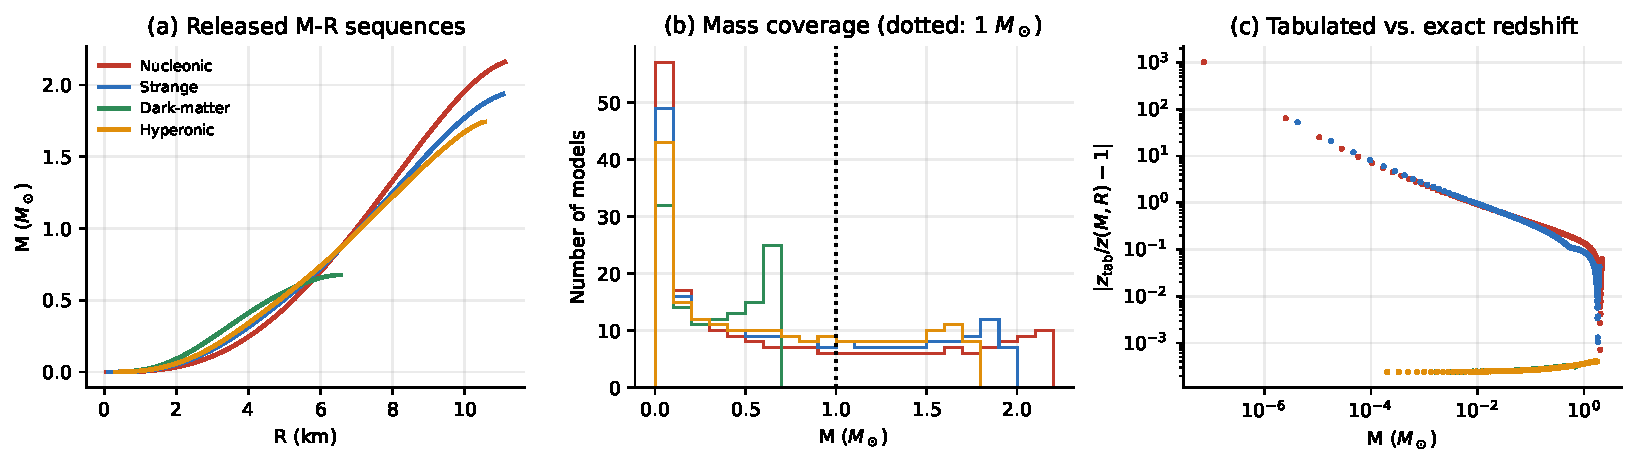
\includegraphics[width=\textwidth]{figs/fig1_data_audit.pdf}
\caption{(a) Mass--radius sequences of the four classes. (b) Distribution of masses; the dotted line is $1\,\Msun$. (c) Fractional difference between the tabulated surface redshift and the value implied by $M$ and $R$; the hyperonic and dark-matter classes agree to $\sim\!0.03\%$, the nucleonic and strange classes do not.}\label{fig:audit}\end{figure}
\begin{enumerate}
\item \emph{Class sizes.} The classes contain 222, 220, 122 and 206 models (not $\approx190$ each).
\item \emph{Sampling.} Models lie on a regular radius grid ($\Delta R=0.05$\,km) along each sequence, so neighbouring models are almost identical: for 96.5\% of the models the nearest neighbour in standardised $(\ln M,\ln R,\ln f,\ln\tau)$ belongs to the same class.
\item \emph{Mass coverage.} 49\% of the models have $M<0.5\,\Msun$ and 70\% have $M<1\,\Msun$, down to $7.2\times10^{-8}\,\Msun$.
\item \emph{The dark-matter sequence ends at $0.68\,\Msun$,} so at $M\gtrsim0.7\,\Msun$ the class is excluded by the mass alone.
\item \emph{Redshift inconsistency.} For the dark-matter and hyperonic classes the tabulated $z$ equals the Schwarzschild value implied by $(M,R)$ to $\approx$0.031\%; for the nucleonic and strange classes the median deviation is +18\% and +11\%. A logistic regression on the redshift residual alone separates \{nucleonic, strange\} from \{dark matter, hyperonic\} with 91\% cross-validated accuracy (57\% for $M$ alone, 72\% for $M$ and $R$). The redshift is therefore a class-dependent artefact and is not used in any analysis here.
\end{enumerate}


\subsection{Replicating the earlier protocol}\label{sec:repro}
Table~\ref{tab:repro} and Fig.~\ref{fig:repro} repeat the earlier random-split protocol for 100 seeds. The published 97.4\% is typical ($97.7\pm1.6\%$), so it is reproducible, but it is not specific to the MLP: a random forest reaches 99.2\%. Removing the redshift changes the MLP result only from 97.7\% to 97.5\%. With $M$ and $R$ only, a $k$-nearest-neighbour classifier reaches 60.1\%, and with $M$ alone logistic regression is at chance (25.3\%).
\begin{table}[t]\centering\small
\caption{Random-split test accuracy (\%) over 100 seeds (stratified 70/15/15, $N_{\rm test}=116$), noise-free.}\label{tab:repro}
\begin{tabular}{lrrr}\toprule Setup & Mean & s.d. & Min--max\\\midrulePublished setup: 7 columns incl.\ $z$, MLP & 97.7 & 1.6 & 92.2--100.0 \\
Published setup, random forest & 99.2 & 1.1 & 94.0--100.0 \\
Redshift removed, MLP & 97.5 & 1.9 & 90.5--100.0 \\
Redshift removed, random forest & 98.9 & 1.2 & 94.0--100.0 \\
Redshift removed, $k$-NN & 98.7 & 1.0 & 96.6--100.0 \\
$M,R,f,\tau$ only, MLP & 93.6 & 3.5 & 79.3--99.1 \\
$M,R$ only, $k$-NN & 60.1 & 4.1 & 50.9--69.8 \\
$M,R$ only, logistic regression & 27.1 & 4.0 & 19.0--41.4 \\
$M$ only, logistic regression & 25.3 & 3.4 & 15.5--31.9\\\bottomrule\end{tabular}\end{table}
\begin{figure}[t]\centering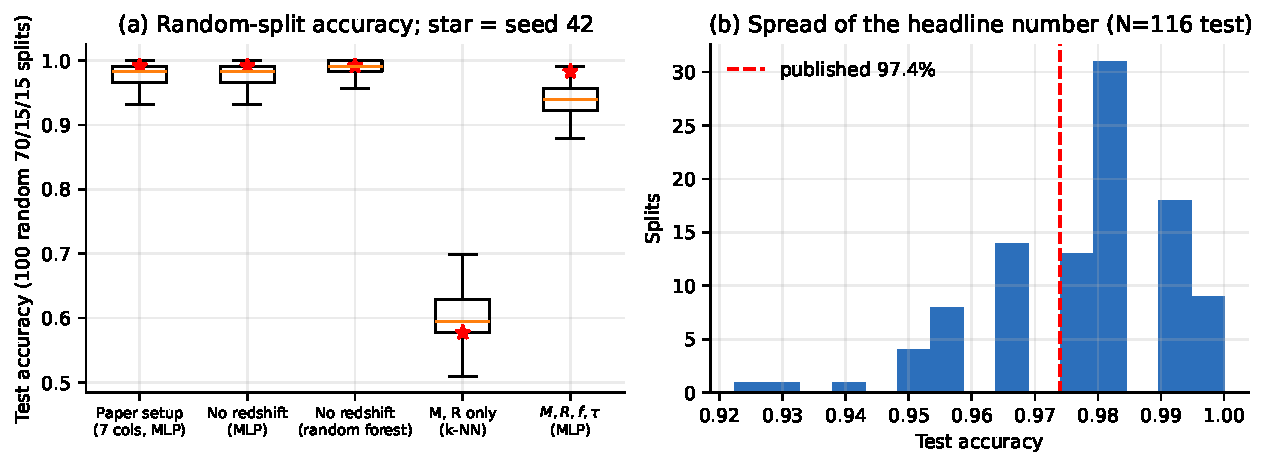
\includegraphics[width=.92\textwidth]{figs/fig2_repro.pdf}
\caption{(a) Test accuracy over 100 random splits for several setups (star: seed 42, used in the earlier version). (b) Distribution for the original setup.}\label{fig:repro}\end{figure}


\subsection{Noise study}
\paragraph{Mass regimes, errors, learners, oracle.}
Three mass regimes are used: \textbf{A}, all models ($N=770$); \textbf{B}, $M\ge0.5\,\Msun$ ($N=395$, with 40 dark-matter models); \textbf{C}, $M\ge1\,\Msun$ ($N=232$, three classes). Contiguous mass blocks of six models are assigned at random to training (60\%), calibration (20\%) and test (20\%) roles; the analysis is repeated for 10 random assignments. Observables are perturbed as $x_j(1+s\sigma_j\epsilon_j)$ with $(\sigma_M,\sigma_R,\sigma_f,\sigma_\tau)=(5,5,2,20)\%$ at $s=1$. The learner is a three-member MLP ensemble, with logistic regression and a random forest as baselines. The oracle Bayes classifier knows the exact sequences (including the test blocks) and the error model,
\begin{equation}
P(k\mid\mathbf x^{\rm obs})\;\propto\;\frac1{N_k}\sum_{i\in k}\;\prod_j \mathcal N\!\left(x^{\rm obs}_j;\,x_{ij},\,(s\sigma_j x_{ij})^2\right),
\end{equation}
and is an upper bound for learners trained on finite data.

\paragraph{Results.}
At $s=1$ in regime B the ensemble reaches 47\% with $\ftau$ against an oracle ceiling of 65\% (chance 25\%); $M$ and $R$ alone give 29\% (oracle 49\%). In regime C (three classes) the values are 50\% (ensemble) and 65\% (oracle). Adding $f$ raises the oracle from 49\% to 64\%; adding a 20\% $\tau$ gives 65\%. Strange and hyperonic matter are the most confused pair (36\% of strange models labelled hyperonic and 37\% the reverse). The raw ensemble is overconfident (ECE 0.188, NLL 1.13 at $s=1$, regime B; oracle 0.040, 0.74); temperature scaling reduces them to 0.096 and 1.00. Conformal sets have about 90\% marginal coverage and contain 2.35 of four classes at $s=1$ (oracle 1.85). When the heaviest 25\% of each class is withheld, the ensemble reaches 50\% (oracle 80\%) and the conformal sets cover only 0.81, since exchangeability fails; the ensemble's mutual information rises from 0.010 to 0.025 nats, an incomplete warning.
\begin{figure}[t]\centering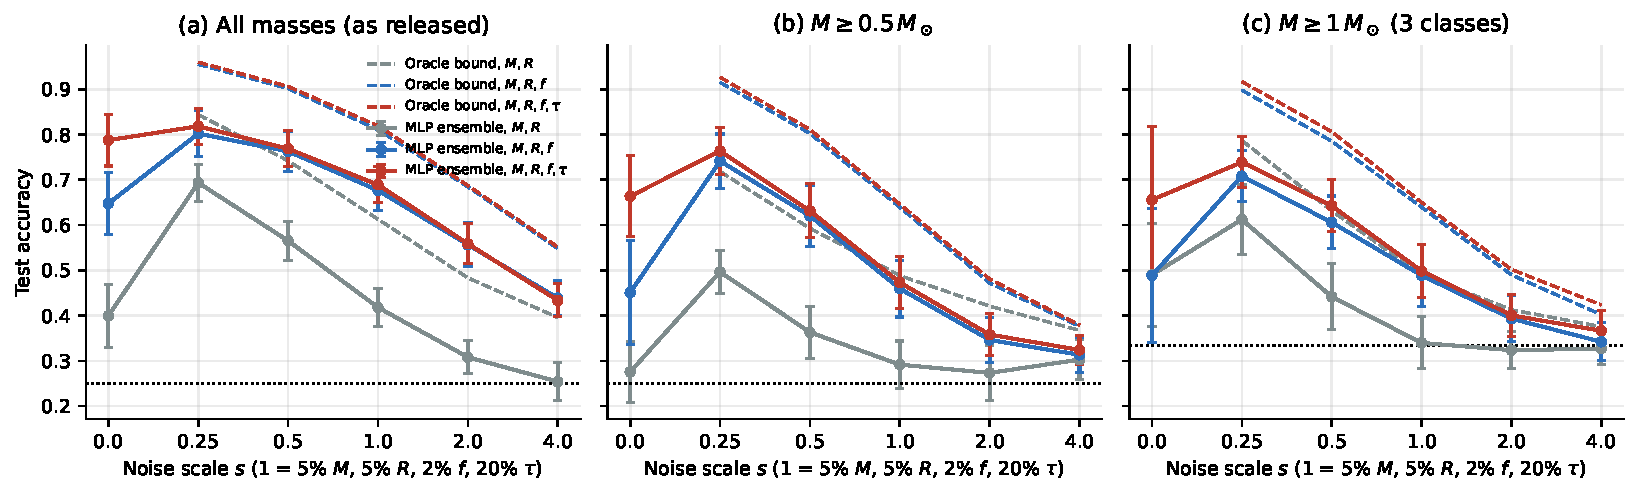
\includegraphics[width=\textwidth]{figs/fig4_noise.pdf}
\caption{Single-sequence data: test accuracy versus noise scale $s$ for the MLP ensemble (solid, 95\% $t$-intervals over 10 repetitions) and the oracle Bayes bound (dashed). Dotted: chance.}\label{fig:noise}\end{figure}
\begin{table}[t]\centering\footnotesize
\caption{Single-sequence data: test accuracy (\%, mean $\pm$ 95\% $t$-interval over 10 repetitions) by regime, observable set and noise scale $s$. Chance is 25\% (A, B) or 33\% (C).}\label{tab:main}
\begin{tabular}{llrcccc}\toprule
Regime & Observables & $s$ & MLP ensemble & Logistic reg. & Random forest & Oracle bound\\\midrule
A & $M,R$ & 0.25 & 69.4$\pm$4.0 & 35.9$\pm$5.4 & 21.3$\pm$3.5 & 84.4$\pm$2.7 \\
A & $M,R$ & 1 & 41.8$\pm$4.2 & 37.1$\pm$4.5 & 24.8$\pm$3.5 & 61.3$\pm$4.2 \\
A & $M,R$ & 4 & 25.4$\pm$4.2 & 29.1$\pm$3.7 & 23.1$\pm$2.5 & 39.6$\pm$4.1 \\
A & $M,R,f$ & 0.25 & 80.2$\pm$5.1 & 38.7$\pm$4.9 & 56.0$\pm$4.9 & 95.5$\pm$1.1 \\
A & $M,R,f$ & 1 & 67.7$\pm$4.4 & 38.7$\pm$5.2 & 56.3$\pm$3.5 & 81.1$\pm$2.8 \\
A & $M,R,f$ & 4 & 43.9$\pm$3.8 & 38.3$\pm$4.3 & 39.5$\pm$2.7 & 54.8$\pm$3.3 \\
A & $M,R,f,\tau$ & 0.25 & 81.8$\pm$4.0 & 44.8$\pm$4.8 & 58.9$\pm$3.7 & 96.0$\pm$1.0 \\
A & $M,R,f,\tau$ & 1 & 68.9$\pm$4.0 & 40.3$\pm$4.3 & 59.6$\pm$3.8 & 81.9$\pm$2.8 \\
A & $M,R,f,\tau$ & 4 & 43.4$\pm$3.7 & 37.8$\pm$4.2 & 39.4$\pm$2.9 & 55.1$\pm$3.1 \\
\midrule
B & $M,R$ & 0.25 & 49.7$\pm$4.8 & 40.6$\pm$6.0 & 30.9$\pm$4.7 & 71.8$\pm$3.9 \\
B & $M,R$ & 1 & 29.2$\pm$5.2 & 35.9$\pm$5.7 & 28.1$\pm$3.5 & 48.8$\pm$2.4 \\
B & $M,R$ & 4 & 30.3$\pm$4.4 & 32.1$\pm$4.3 & 30.1$\pm$1.6 & 36.7$\pm$2.5 \\
B & $M,R,f$ & 0.25 & 74.1$\pm$6.0 & 59.5$\pm$5.2 & 40.8$\pm$5.8 & 91.5$\pm$1.9 \\
B & $M,R,f$ & 1 & 46.0$\pm$6.3 & 45.5$\pm$4.3 & 38.8$\pm$3.8 & 63.9$\pm$2.5 \\
B & $M,R,f$ & 4 & 31.3$\pm$3.9 & 35.1$\pm$4.3 & 30.6$\pm$2.6 & 37.6$\pm$2.2 \\
B & $M,R,f,\tau$ & 0.25 & 76.3$\pm$5.2 & 63.6$\pm$3.9 & 43.4$\pm$5.7 & 92.7$\pm$1.8 \\
B & $M,R,f,\tau$ & 1 & 47.3$\pm$5.8 & 46.4$\pm$4.4 & 39.9$\pm$4.3 & 64.6$\pm$2.7 \\
B & $M,R,f,\tau$ & 4 & 32.4$\pm$3.2 & 35.4$\pm$4.2 & 31.8$\pm$2.2 & 37.9$\pm$2.1 \\
\midrule
C & $M,R$ & 0.25 & 61.2$\pm$7.7 & 62.6$\pm$7.5 & 37.7$\pm$8.7 & 78.7$\pm$4.2 \\
C & $M,R$ & 1 & 34.0$\pm$5.7 & 40.7$\pm$7.1 & 33.1$\pm$5.5 & 49.0$\pm$4.8 \\
C & $M,R$ & 4 & 32.7$\pm$3.5 & 33.9$\pm$6.2 & 33.2$\pm$2.5 & 37.5$\pm$5.8 \\
C & $M,R,f$ & 0.25 & 70.8$\pm$5.6 & 69.0$\pm$6.7 & 44.1$\pm$10.0 & 89.8$\pm$1.6 \\
C & $M,R,f$ & 1 & 48.9$\pm$6.8 & 51.4$\pm$6.6 & 41.9$\pm$6.7 & 64.0$\pm$3.5 \\
C & $M,R,f$ & 4 & 34.2$\pm$4.2 & 36.0$\pm$5.1 & 34.3$\pm$3.4 & 40.2$\pm$4.3 \\
C & $M,R,f,\tau$ & 0.25 & 73.9$\pm$5.6 & 72.5$\pm$6.4 & 50.0$\pm$9.6 & 91.7$\pm$1.4 \\
C & $M,R,f,\tau$ & 1 & 49.9$\pm$5.9 & 52.5$\pm$7.0 & 44.1$\pm$6.9 & 65.0$\pm$3.1 \\
C & $M,R,f,\tau$ & 4 & 36.6$\pm$4.4 & 36.6$\pm$5.3 & 35.7$\pm$3.1 & 42.4$\pm$4.7\\\bottomrule\end{tabular}\end{table}
\begin{figure}[t]\centering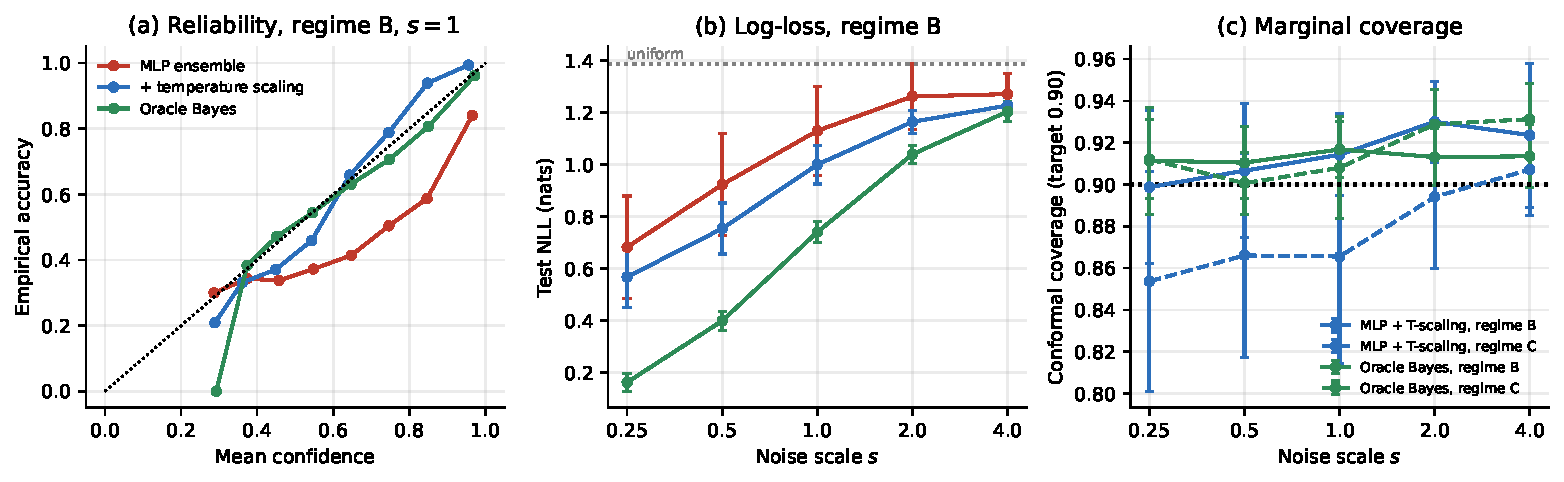
\includegraphics[width=\textwidth]{figs/fig6_uncertainty.pdf}
\caption{Single-sequence data: (a) reliability diagram (regime B, $s=1$), (b) NLL, (c) conformal coverage versus noise scale.}\label{fig:unc}\end{figure}

\section{Experimental settings}\label{sec:settings}
\begin{table}[H]\centering\small\caption{Settings.}
\begin{tabular}{p{.22\textwidth}p{.70\textwidth}}\toprule
Item & Setting\\\midrule
Population folds & 5 folds by EoS (stratified), test / calibration / training = 1 / 1 / 3 folds, 3 random partitions\\
Population samples & training: 33 masses $\times$ 3 noise draws per EoS; calibration: 33 $\times$ 2; test: 33 $\times$ 3 (single draw when noise-free)\\
MLP & 3 members, $2\times64$ ReLU, Adam, lr $10^{-3}$, $\alpha=10^{-4}$, batch 128, early stopping (max 120 iterations)\\
Other learners & logistic regression (L2); $k$-NN, $k=25$; random forest, 200 trees, min leaf 5; histogram gradient boosting (150 iterations); RBF SVM, $C=3$, 8000 samples\\
Kernel Bayes & reference: 22 masses per EoS; training EoS, or all non-test EoS\\
Robustness studies & EoS-level bootstrap: 2000 resamples within class; learning curves: 25, 50, 75, 100\% of the training EoS; population B: 48 EoS per scenario, same folds protocol; out-of-family: train on all EoS of one population, test on all of the other, three noise seeds\\
Numerical tests & integration tolerances $10^{-8}$--$10^{-13}$, surface cut-off $10^{-6}$--$10^{-4}$, centre radius $\times$0.5--2.5, matching radius 1500--8000\,km, crust pressure scale $\pm10\%$\\
Conformal & LAC score, $\alpha=0.1$; one star per calibration EoS (average of 40 random choices), quantile level $\lceil(n+1)(1-\alpha)\rceil/n$ with $n$ the number of calibration EoS; pooled variant as sensitivity check\\
Tuned learners (Sec.~\ref{sec:tuned}) & grids: logistic regression $C\in\{0.1,1,10,100\}$; $k$-NN $k\in\{5,25,100\}$; random forest min.\ leaf $\{1,5,20\}\times$ max.\ features $\{\sqrt{\cdot},\text{all}\}$; gradient boosting depth $\{3,\text{none}\}\times$ learning rate $\{0.05,0.1\}\times$ iterations $\{150,400\}$; SVM $C\in\{1,10,100\}\times\gamma\in\{0.1,0.5,\text{scale}\}$ (6000 samples); MLP $\{(64,64),(128,128,128),(256,256)\}\times\alpha\in\{10^{-4},10^{-2}\}$; selection on the calibration EoS; 2 repetitions of 5 folds\\
Subsets and narrowed priors & nucleonic vs dark matter only; whole-EoS 5-fold, 10 repetitions; balanced accuracy; narrowed windows $w\in\{0.4,0.2,0.1\}$ about the SLy fit, 40 EoS per class and window, five masses per EoS ($1.2,1.4,1.6,1.8,1.9\,\Msun$), $s\in\{0,0.25,1\}$\\
Single-sequence study & blocks of six models, 60/20/20, 10 repetitions; 20 noise draws per training model; random forest 150 trees; 15 repetitions for the block-length study, 100 for the random-split replication\\\bottomrule\end{tabular}\end{table}

\section{Changes relative to arXiv:2512.23758v3}\label{sec:changes}
\begin{table}[H]\centering\small\caption{Statements of the earlier version that are withdrawn or changed.}
\begin{tabular}{p{.42\textwidth}p{.5\textwidth}}\toprule
Earlier statement & Status\\\midrule
Each class is one EoS; the classifier ``separates composition'' & Replaced by populations of EoS with whole-EoS hold-out; the accuracy ceiling is about 65\% and no discrimination between nucleonic and dark-matter-admixed matter is demonstrated.\\
$\approx190$ models per class, 770 in total & Total is correct; classes contain 222, 220, 122 and 206 models.\\
Models span $\sim1\,\Msun$ to the maximum mass & The data span $7\times10^{-8}$ to $2.16\,\Msun$; 70\% have $M<1\,\Msun$.\\
97.4\% test accuracy & Reproducible (97.7\% average over 100 splits) but inflated by neighbouring models; falls to 94--69\% with six- to 24-model blocks.\\
Per-class accuracy ranges 82--97\% ``across dataset realizations'' & Not reproduced; removed.\\
``Mild degradation near the high-mass end'' & Not supported by the earlier figure; removed.\\
``Not merely overfitting noise'' & The inputs were noise-free; replaced by explicit error scenarios.\\
Permutation importance shows $f$ and $\tau$ dominate & Replaced by observable-set ablations: $f$ carries the information, $\tau$ adds nothing.\\
Tabulated redshift used as an input & Inconsistent with $(M,R)$ for two classes; removed.\\
Oscillation quantities from the earlier code & Population data generated with a new solver, checked against six $f$-mode frequencies of an unpublished same-author cross-code pilot, analytic benchmarks and a published damping-time relation.\\\bottomrule\end{tabular}\end{table}

\begin{thebibliography}{99}\small
\bibitem[Abbott et al.(2018)]{Abbott18} B.~P. Abbott et al. (LIGO Scientific and Virgo Collaborations), Phys. Rev. Lett. \textbf{121}, 161101 (2018).
\bibitem[Andersson \& Kokkotas(1998)]{AK98} N. Andersson and K.~D. Kokkotas, Mon. Not. R. Astron. Soc. \textbf{299}, 1059 (1998).
\bibitem[Angelopoulos \& Bates(2023)]{Angelopoulos23} A.~N. Angelopoulos and S. Bates, Found. Trends Mach. Learn. \textbf{16}, 494 (2023) [arXiv:2107.07511].
\bibitem[Baym et al.(2018)]{Baym18} G. Baym, D.~H. Beck, P. Geltenbort, J. Shelton, Phys. Rev. Lett. \textbf{121}, 061801 (2018).
\bibitem[Benhar et al.(2004)]{Benhar04} O. Benhar, V. Ferrari, L. Gualtieri, Phys. Rev. D \textbf{70}, 124015 (2004).
\bibitem[Damour \& Nagar(2009)]{Damour09} T. Damour and A. Nagar, Phys. Rev. D \textbf{80}, 084035 (2009).
\bibitem[Detweiler \& Lindblom(1985)]{DL85} S. Detweiler and L. Lindblom, Astrophys. J. \textbf{292}, 12 (1985).
\bibitem[Ellis et al.(2018)]{Ellis18} J. Ellis, G. H\"utsi, K. Kannike, L. Marzola, M. Raidal, V. Vaskonen, Phys. Rev. D \textbf{97}, 123007 (2018).
\bibitem[Ferreira \& Provid\^encia(2021)]{Ferreira21} M. Ferreira and C. Provid\^encia, J. Cosmol. Astropart. Phys. 07 (2021) 011 [arXiv:1910.05554].
\bibitem[Fornal \& Grinstein(2018)]{FG18} B. Fornal and B. Grinstein, Phys. Rev. Lett. \textbf{120}, 191801 (2018).
\bibitem[Fujimoto et al.(2018)]{Fujimoto18} Y. Fujimoto, K. Fukushima, K. Murase, Phys. Rev. D \textbf{98}, 023019 (2018).
\bibitem[Hinderer(2008)]{Hinderer08} T. Hinderer, Astrophys. J. \textbf{677}, 1216 (2008).
\bibitem[Husain et al.(2022)]{Husain22} W. Husain, S. Motta, A.~W. Thomas, arXiv:2203.02758 (2022).
\bibitem[Husain(2025)]{Husain25} W. Husain, \emph{F-mode oscillations of neutron stars with dark matter from neutron decay: implications for gravitational-wave detectability}, arXiv:2505.17355 (published in Phys. Dark Universe \textbf{51}, 2026).
\bibitem[Husain(2026)]{HusainPilot} W. Husain, \emph{Testing f-mode information beyond static structure in neutron-decay dark-matter stars: a finite-EoS pilot and working research manuscript}, 15 October 2026 (unpublished working manuscript).
\bibitem[Lakshminarayanan et al.(2017)]{Lakshminarayanan17} B. Lakshminarayanan, A. Pritzel, C. Blundell, Adv. Neural Inf. Process. Syst. \textbf{30} (2017).
\bibitem[Lattimer \& Prakash(2004)]{LP04} J.~M. Lattimer and M. Prakash, Science \textbf{304}, 536 (2004).
\bibitem[Leaver(1985)]{Leaver85} E.~W. Leaver, Proc. R. Soc. Lond. A \textbf{402}, 285 (1985).
\bibitem[Leung et al.(2011)]{Leung11} S.-C. Leung, M.-C. Chu, L.-M. Lin, Phys. Rev. D \textbf{84}, 107301 (2011).
\bibitem[Lioutas \& Stergioulas(2018)]{LS18} G. Lioutas and N. Stergioulas, Gen. Relativ. Gravit. \textbf{50}, 12 (2018) [arXiv:1709.10067].
\bibitem[McKeen et al.(2018)]{McKeen18} D. McKeen, A.~E. Nelson, S. Reddy, D. Zhou, Phys. Rev. Lett. \textbf{121}, 061802 (2018).
\bibitem[Miller et al.(2019)]{Miller19} M.~C. Miller et al., Astrophys. J. Lett. \textbf{887}, L24 (2019).
\bibitem[Motta et al.(2018)]{Motta18} T.~F. Motta, P.~A.~M. Guichon, A.~W. Thomas, J. Phys. G \textbf{45}, 05LT01 (2018).
\bibitem[Oppenheimer \& Volkoff(1939)]{OV39} J.~R. Oppenheimer and G.~M. Volkoff, Phys. Rev. \textbf{55}, 374 (1939).
\bibitem[\"Ozel \& Freire(2016)]{OF16} F. \"Ozel and P. Freire, Annu. Rev. Astron. Astrophys. \textbf{54}, 401 (2016).
\bibitem[Postnikov et al.(2010)]{Postnikov10} S. Postnikov, M. Prakash, J.~M. Lattimer, Phys. Rev. D \textbf{82}, 024016 (2010).
\bibitem[Read et al.(2009)]{Read09} J.~S. Read, B.~D. Lackey, B.~J. Owen, J.~L. Friedman, Phys. Rev. D \textbf{79}, 124032 (2009).
\bibitem[Rikovska Stone et al.(2007)]{Stone07} J. Rikovska Stone, P.~A.~M. Guichon, H.~H. Matevosyan, A.~W. Thomas, Nucl. Phys. A \textbf{792}, 341 (2007).
\bibitem[Riley et al.(2019)]{Riley19} T.~E. Riley et al., Astrophys. J. Lett. \textbf{887}, L21 (2019).
\bibitem[Tolman(1939)]{Tolman39} R.~C. Tolman, Phys. Rev. \textbf{55}, 364 (1939).
\bibitem[Vovk et al.(2005)]{Vovk05} V. Vovk, A. Gammerman, G. Shafer, \emph{Algorithmic Learning in a Random World} (Springer, 2005).
\bibitem[Williams et al.(2022)]{Williams22} N. Williams, G. Pratten, P. Schmidt, Phys. Rev. D \textbf{105}, 123032 (2022) [arXiv:2203.00623].
\bibitem[Zerilli(1970)]{Zerilli70} F.~J. Zerilli, Phys. Rev. D \textbf{2}, 2141 (1970).
\end{thebibliography}
\end{document}
